\documentclass[twoside]{book}

% Packages required by doxygen
\usepackage{calc}
\usepackage{doxygen}
\usepackage{graphicx}
\usepackage[utf8]{inputenc}
\usepackage{makeidx}
\usepackage{multicol}
\usepackage{multirow}
\usepackage{textcomp}
\usepackage[table]{xcolor}

% Font selection
\usepackage[T1]{fontenc}
\usepackage{mathptmx}
\usepackage[scaled=.90]{helvet}
\usepackage{courier}
\usepackage{amssymb}
\usepackage{sectsty}
\renewcommand{\familydefault}{\sfdefault}
\allsectionsfont{%
  \fontseries{bc}\selectfont%
  \color{darkgray}%
}
\renewcommand{\DoxyLabelFont}{%
  \fontseries{bc}\selectfont%
  \color{darkgray}%
}

% Page & text layout
\usepackage{geometry}
\geometry{%
  a4paper,%
  top=2.5cm,%
  bottom=2.5cm,%
  left=2.5cm,%
  right=2.5cm%
}
\tolerance=750
\hfuzz=15pt
\hbadness=750
\setlength{\emergencystretch}{15pt}
\setlength{\parindent}{0cm}
\setlength{\parskip}{0.2cm}
\makeatletter
\renewcommand{\paragraph}{%
  \@startsection{paragraph}{4}{0ex}{-1.0ex}{1.0ex}{%
    \normalfont\normalsize\bfseries\SS@parafont%
  }%
}
\renewcommand{\subparagraph}{%
  \@startsection{subparagraph}{5}{0ex}{-1.0ex}{1.0ex}{%
    \normalfont\normalsize\bfseries\SS@subparafont%
  }%
}
\makeatother

% Headers & footers
\usepackage{fancyhdr}
\pagestyle{fancyplain}
\fancyhead[LE]{\fancyplain{}{\bfseries\thepage}}
\fancyhead[CE]{\fancyplain{}{}}
\fancyhead[RE]{\fancyplain{}{\bfseries\leftmark}}
\fancyhead[LO]{\fancyplain{}{\bfseries\rightmark}}
\fancyhead[CO]{\fancyplain{}{}}
\fancyhead[RO]{\fancyplain{}{\bfseries\thepage}}
\fancyfoot[LE]{\fancyplain{}{}}
\fancyfoot[CE]{\fancyplain{}{}}
\fancyfoot[RE]{\fancyplain{}{\bfseries\scriptsize Generated on Thu Jun 8 2017 10\-:44\-:05 for Maze by Doxygen }}
\fancyfoot[LO]{\fancyplain{}{\bfseries\scriptsize Generated on Thu Jun 8 2017 10\-:44\-:05 for Maze by Doxygen }}
\fancyfoot[CO]{\fancyplain{}{}}
\fancyfoot[RO]{\fancyplain{}{}}
\renewcommand{\footrulewidth}{0.4pt}
\renewcommand{\chaptermark}[1]{%
  \markboth{#1}{}%
}
\renewcommand{\sectionmark}[1]{%
  \markright{\thesection\ #1}%
}

% Indices & bibliography
\usepackage{natbib}
\usepackage[titles]{tocloft}
\setcounter{tocdepth}{3}
\setcounter{secnumdepth}{5}
\makeindex

% Hyperlinks (required, but should be loaded last)
\usepackage{ifpdf}
\ifpdf
  \usepackage[pdftex,pagebackref=true]{hyperref}
\else
  \usepackage[ps2pdf,pagebackref=true]{hyperref}
\fi
\hypersetup{%
  colorlinks=true,%
  linkcolor=blue,%
  citecolor=blue,%
  unicode%
}

% Custom commands
\newcommand{\clearemptydoublepage}{%
  \newpage{\pagestyle{empty}\cleardoublepage}%
}


%===== C O N T E N T S =====

\begin{document}

% Titlepage & ToC
\hypersetup{pageanchor=false}
\pagenumbering{roman}
\begin{titlepage}
\vspace*{7cm}
\begin{center}%
{\Large Maze }\\
\vspace*{1cm}
{\large Generated by Doxygen 1.8.6}\\
\vspace*{0.5cm}
{\small Thu Jun 8 2017 10:44:05}\\
\end{center}
\end{titlepage}
\clearemptydoublepage
\tableofcontents
\clearemptydoublepage
\pagenumbering{arabic}
\hypersetup{pageanchor=true}

%--- Begin generated contents ---
\chapter{Namespace Index}
\section{Namespace List}
Here is a list of all namespaces with brief descriptions\-:\begin{DoxyCompactList}
\item\contentsline{section}{\hyperlink{namespace_ui}{Ui} }{\pageref{namespace_ui}}{}
\end{DoxyCompactList}

\chapter{Hierarchical Index}
\section{Class Hierarchy}
This inheritance list is sorted roughly, but not completely, alphabetically\-:\begin{DoxyCompactList}
\item \contentsline{section}{Breadth\-First\-Search}{\pageref{class_breadth_first_search}}{}
\item \contentsline{section}{Maze}{\pageref{class_maze}}{}
\item \contentsline{section}{Maze\-Generator}{\pageref{class_maze_generator}}{}
\item \contentsline{section}{Position}{\pageref{class_position}}{}
\item Q\-Main\-Window\begin{DoxyCompactList}
\item \contentsline{section}{Maze\-Gui}{\pageref{class_maze_gui}}{}
\end{DoxyCompactList}
\item Q\-Thread\begin{DoxyCompactList}
\item \contentsline{section}{Maze\-Solve\-Algorithm}{\pageref{class_maze_solve_algorithm}}{}
\begin{DoxyCompactList}
\item \contentsline{section}{Breadth\-First\-Search\-Gui\-Interaction}{\pageref{class_breadth_first_search_gui_interaction}}{}
\item \contentsline{section}{Recursive\-Maze\-Solve\-Algorithm}{\pageref{class_recursive_maze_solve_algorithm}}{}
\end{DoxyCompactList}
\end{DoxyCompactList}
\end{DoxyCompactList}

\chapter{Class Index}
\section{Class List}
Here are the classes, structs, unions and interfaces with brief descriptions\-:\begin{DoxyCompactList}
\item\contentsline{section}{\hyperlink{class_breadth_first_search}{Breadth\-First\-Search} \\*Algorithm to find shortest way through maze by using breadth fist search }{\pageref{class_breadth_first_search}}{}
\item\contentsline{section}{\hyperlink{class_breadth_first_search_gui_interaction}{Breadth\-First\-Search\-Gui\-Interaction} \\*Wraps logic of Breath\-First\-Search into class extending \hyperlink{class_maze_solve_algorithm}{Maze\-Solve\-Algorithm} }{\pageref{class_breadth_first_search_gui_interaction}}{}
\item\contentsline{section}{\hyperlink{class_maze}{Maze} \\*Model of the maze with functions to set an get fields of the maze }{\pageref{class_maze}}{}
\item\contentsline{section}{\hyperlink{class_maze_generator}{Maze\-Generator} }{\pageref{class_maze_generator}}{}
\item\contentsline{section}{\hyperlink{class_maze_gui}{Maze\-Gui} }{\pageref{class_maze_gui}}{}
\item\contentsline{section}{\hyperlink{class_maze_solve_algorithm}{Maze\-Solve\-Algorithm} \\*The Maze\-Algorithm class Baseclass have to be derived by all maze solve algorithm classes contains the datastructures for the maze such as methods to redrow }{\pageref{class_maze_solve_algorithm}}{}
\item\contentsline{section}{\hyperlink{class_position}{Position} \\*Structure allowing to exchange positions with two dimensions }{\pageref{class_position}}{}
\item\contentsline{section}{\hyperlink{class_recursive_maze_solve_algorithm}{Recursive\-Maze\-Solve\-Algorithm} }{\pageref{class_recursive_maze_solve_algorithm}}{}
\end{DoxyCompactList}

\chapter{File Index}
\section{File List}
Here is a list of all files with brief descriptions\-:\begin{DoxyCompactList}
\item\contentsline{section}{/home/travis/build/algdat/blatt-\/2-\/maze/src/ss17/algodat/maze/\hyperlink{main_8cpp}{main.\-cpp} }{\pageref{main_8cpp}}{}
\item\contentsline{section}{/home/travis/build/algdat/blatt-\/2-\/maze/src/ss17/algodat/maze/control/\hyperlink{mazealgorithm_8cpp}{mazealgorithm.\-cpp} }{\pageref{mazealgorithm_8cpp}}{}
\item\contentsline{section}{/home/travis/build/algdat/blatt-\/2-\/maze/src/ss17/algodat/maze/control/\hyperlink{mazealgorithm_8h}{mazealgorithm.\-h} }{\pageref{mazealgorithm_8h}}{}
\item\contentsline{section}{/home/travis/build/algdat/blatt-\/2-\/maze/src/ss17/algodat/maze/control/\hyperlink{mazegenerator_8cpp}{mazegenerator.\-cpp} }{\pageref{mazegenerator_8cpp}}{}
\item\contentsline{section}{/home/travis/build/algdat/blatt-\/2-\/maze/src/ss17/algodat/maze/control/\hyperlink{mazegenerator_8h}{mazegenerator.\-h} }{\pageref{mazegenerator_8h}}{}
\item\contentsline{section}{/home/travis/build/algdat/blatt-\/2-\/maze/src/ss17/algodat/maze/control/recursive\-\_\-solver/\hyperlink{recursivemazesolvealgorithm_8cpp}{recursivemazesolvealgorithm.\-cpp} }{\pageref{recursivemazesolvealgorithm_8cpp}}{}
\item\contentsline{section}{/home/travis/build/algdat/blatt-\/2-\/maze/src/ss17/algodat/maze/control/recursive\-\_\-solver/\hyperlink{recursivemazesolvealgorithm_8h}{recursivemazesolvealgorithm.\-h} }{\pageref{recursivemazesolvealgorithm_8h}}{}
\item\contentsline{section}{/home/travis/build/algdat/blatt-\/2-\/maze/src/ss17/algodat/maze/control/shortest\-\_\-path/breadth\-\_\-first\-\_\-search/\hyperlink{_breadth_first_search_8cpp}{Breadth\-First\-Search.\-cpp} }{\pageref{_breadth_first_search_8cpp}}{}
\item\contentsline{section}{/home/travis/build/algdat/blatt-\/2-\/maze/src/ss17/algodat/maze/control/shortest\-\_\-path/breadth\-\_\-first\-\_\-search/\hyperlink{_breadth_first_search_8h}{Breadth\-First\-Search.\-h} }{\pageref{_breadth_first_search_8h}}{}
\item\contentsline{section}{/home/travis/build/algdat/blatt-\/2-\/maze/src/ss17/algodat/maze/control/shortest\-\_\-path/breadth\-\_\-first\-\_\-search/\hyperlink{_breadth_first_search_gui_interaction_8cpp}{Breadth\-First\-Search\-Gui\-Interaction.\-cpp} }{\pageref{_breadth_first_search_gui_interaction_8cpp}}{}
\item\contentsline{section}{/home/travis/build/algdat/blatt-\/2-\/maze/src/ss17/algodat/maze/control/shortest\-\_\-path/breadth\-\_\-first\-\_\-search/\hyperlink{_breadth_first_search_gui_interaction_8h}{Breadth\-First\-Search\-Gui\-Interaction.\-h} }{\pageref{_breadth_first_search_gui_interaction_8h}}{}
\item\contentsline{section}{/home/travis/build/algdat/blatt-\/2-\/maze/src/ss17/algodat/maze/control/shortest\-\_\-path/breadth\-\_\-first\-\_\-search/\hyperlink{_position_8cpp}{Position.\-cpp} }{\pageref{_position_8cpp}}{}
\item\contentsline{section}{/home/travis/build/algdat/blatt-\/2-\/maze/src/ss17/algodat/maze/control/shortest\-\_\-path/breadth\-\_\-first\-\_\-search/\hyperlink{_position_8h}{Position.\-h} }{\pageref{_position_8h}}{}
\item\contentsline{section}{/home/travis/build/algdat/blatt-\/2-\/maze/src/ss17/algodat/maze/model/\hyperlink{maze_8cpp}{maze.\-cpp} }{\pageref{maze_8cpp}}{}
\item\contentsline{section}{/home/travis/build/algdat/blatt-\/2-\/maze/src/ss17/algodat/maze/model/\hyperlink{maze_8h}{maze.\-h} }{\pageref{maze_8h}}{}
\item\contentsline{section}{/home/travis/build/algdat/blatt-\/2-\/maze/src/ss17/algodat/maze/view/\hyperlink{mazegui_8cpp}{mazegui.\-cpp} }{\pageref{mazegui_8cpp}}{}
\item\contentsline{section}{/home/travis/build/algdat/blatt-\/2-\/maze/src/ss17/algodat/maze/view/\hyperlink{mazegui_8h}{mazegui.\-h} }{\pageref{mazegui_8h}}{}
\end{DoxyCompactList}

\chapter{Namespace Documentation}
\hypertarget{namespace_ui}{\section{Ui Namespace Reference}
\label{namespace_ui}\index{Ui@{Ui}}
}

\chapter{Class Documentation}
\hypertarget{class_breadth_first_search}{\section{Breadth\-First\-Search Class Reference}
\label{class_breadth_first_search}\index{Breadth\-First\-Search@{Breadth\-First\-Search}}
}


Algorithm to find shortest way through maze by using breadth fist search.  




{\ttfamily \#include $<$Breadth\-First\-Search.\-h$>$}

\subsection*{Public Member Functions}
\begin{DoxyCompactItemize}
\item 
\hyperlink{class_breadth_first_search_aa2eb988878d47abbb9a75de86dd3ccb6}{Breadth\-First\-Search} (\hyperlink{class_maze}{Maze} $\ast$maze)
\item 
\hyperlink{class_breadth_first_search_af56e60466779aa47b1b3c10a1a84d8ca}{$\sim$\-Breadth\-First\-Search} ()
\item 
bool \hyperlink{class_breadth_first_search_a0fccce0a839583c2e80eaacc1be8ed2e}{solve} (int \&steps)
\item 
void \hyperlink{class_breadth_first_search_a466d9907ad4223398e65c56743c887fe}{push\-Free\-Adjacent\-Fields} (\hyperlink{class_position}{Position} $\ast$position)
\item 
void \hyperlink{class_breadth_first_search_a71c86843e6fd1927280edbbb8fef9c23}{consume\-Position} ()
\item 
void \hyperlink{class_breadth_first_search_aff710f432b18251df00018f9a1603f19}{plot\-Solution} (\hyperlink{class_position}{Position} position)
\item 
void \hyperlink{class_breadth_first_search_a83527ad23d6f10bea0a91fe0aad1056d}{consume\-Field} (\hyperlink{class_position}{Position} position, const int column\-Offset, const int row\-Offset)
\item 
\hyperlink{class_position}{Position} $\ast$ \hyperlink{class_breadth_first_search_a31746f6d04a82b21a8c81a320fa61023}{search\-For\-Next\-Field\-On\-Shortest\-Path} (\hyperlink{class_position}{Position} position, int steps) const 
\item 
int $\ast$ \hyperlink{class_breadth_first_search_a5e5e17159bdda443af254af3f793b80f}{get\-Solution} () const 
\item 
queue$<$ \hyperlink{class_position}{Position} $>$ $\ast$ \hyperlink{class_breadth_first_search_af5345d1f260e617dc3d1d0636341a71c}{get\-Position\-Queue} () const 
\item 
\hyperlink{class_position}{Position} $\ast$ \hyperlink{class_breadth_first_search_a72d8df8632e4b6bc86afea0793025a48}{get\-Last\-Field} () const 
\item 
int \hyperlink{class_breadth_first_search_a36963ae576749a6aa36f2075f757b925}{get\-Length\-Of\-Shortest\-Path} () const 
\end{DoxyCompactItemize}
\subsection*{Static Public Member Functions}
\begin{DoxyCompactItemize}
\item 
static int \hyperlink{class_breadth_first_search_a1e5271b5561e4fe52b7e67917f72511e}{get\-Field} (const int C\-O\-L\-U\-M\-N\-S, const int R\-O\-W\-S, int $\ast$matrix, const int column, const int row)
\item 
static \hyperlink{class_position}{Position} $\ast$ \hyperlink{class_breadth_first_search_a533670621ed3c1e3bfba89d667dab4c3}{get\-Start\-Pos} (const int C\-O\-L\-U\-M\-N\-S, const int R\-O\-W\-S, \hyperlink{class_maze}{Maze} $\ast$maze, const int S\-T\-A\-R\-T\-\_\-\-I\-D)
\item 
static void \hyperlink{class_breadth_first_search_a29e052c3dd62782fabc59a68ef27cade}{set\-Field} (const int C\-O\-L\-U\-M\-N\-S, const int R\-O\-W\-S, int $\ast$matrix, const int column, const int row, int $\ast$content)
\end{DoxyCompactItemize}


\subsection{Detailed Description}
Algorithm to find shortest way through maze by using breadth fist search. 

\subsection{Constructor \& Destructor Documentation}
\hypertarget{class_breadth_first_search_aa2eb988878d47abbb9a75de86dd3ccb6}{\index{Breadth\-First\-Search@{Breadth\-First\-Search}!Breadth\-First\-Search@{Breadth\-First\-Search}}
\index{Breadth\-First\-Search@{Breadth\-First\-Search}!BreadthFirstSearch@{Breadth\-First\-Search}}
\subsubsection[{Breadth\-First\-Search}]{\setlength{\rightskip}{0pt plus 5cm}Breadth\-First\-Search\-::\-Breadth\-First\-Search (
\begin{DoxyParamCaption}
\item[{{\bf Maze} $\ast$}]{maze}
\end{DoxyParamCaption}
)}}\label{class_breadth_first_search_aa2eb988878d47abbb9a75de86dd3ccb6}
Initializes the breadth first search. 
\begin{DoxyParams}{Parameters}
{\em maze} & \hyperlink{class_maze}{Maze} to be solved. \\
\hline
\end{DoxyParams}
\hypertarget{class_breadth_first_search_af56e60466779aa47b1b3c10a1a84d8ca}{\index{Breadth\-First\-Search@{Breadth\-First\-Search}!$\sim$\-Breadth\-First\-Search@{$\sim$\-Breadth\-First\-Search}}
\index{$\sim$\-Breadth\-First\-Search@{$\sim$\-Breadth\-First\-Search}!BreadthFirstSearch@{Breadth\-First\-Search}}
\subsubsection[{$\sim$\-Breadth\-First\-Search}]{\setlength{\rightskip}{0pt plus 5cm}Breadth\-First\-Search\-::$\sim$\-Breadth\-First\-Search (
\begin{DoxyParamCaption}
{}
\end{DoxyParamCaption}
)}}\label{class_breadth_first_search_af56e60466779aa47b1b3c10a1a84d8ca}
Deletes all objects associated to the algorithm from the heap. 

\subsection{Member Function Documentation}
\hypertarget{class_breadth_first_search_a83527ad23d6f10bea0a91fe0aad1056d}{\index{Breadth\-First\-Search@{Breadth\-First\-Search}!consume\-Field@{consume\-Field}}
\index{consume\-Field@{consume\-Field}!BreadthFirstSearch@{Breadth\-First\-Search}}
\subsubsection[{consume\-Field}]{\setlength{\rightskip}{0pt plus 5cm}void Breadth\-First\-Search\-::consume\-Field (
\begin{DoxyParamCaption}
\item[{{\bf Position}}]{position, }
\item[{const int}]{column\-Offset, }
\item[{const int}]{row\-Offset}
\end{DoxyParamCaption}
)}}\label{class_breadth_first_search_a83527ad23d6f10bea0a91fe0aad1056d}
A field given via position plus offset is checked for being open or the goal. If the field is open it will be added to the queue and the number of steps required to reach it will be wrote to it. If it is the goal this will be communicated by setting last\-Field to position. 
\begin{DoxyParams}{Parameters}
{\em position} & Base position. \\
\hline
{\em column\-Offset} & Adding this offset to the column-\/index of position will give the column-\/index of the field to check. \\
\hline
{\em row\-Offset} & Adding this offset to the row-\/index of position will give the row-\/index of the field to check. \\
\hline
{\em maze} & \hyperlink{class_maze}{Maze} to be solved. \\
\hline
\end{DoxyParams}
\hypertarget{class_breadth_first_search_a71c86843e6fd1927280edbbb8fef9c23}{\index{Breadth\-First\-Search@{Breadth\-First\-Search}!consume\-Position@{consume\-Position}}
\index{consume\-Position@{consume\-Position}!BreadthFirstSearch@{Breadth\-First\-Search}}
\subsubsection[{consume\-Position}]{\setlength{\rightskip}{0pt plus 5cm}void Breadth\-First\-Search\-::consume\-Position (
\begin{DoxyParamCaption}
{}
\end{DoxyParamCaption}
)}}\label{class_breadth_first_search_a71c86843e6fd1927280edbbb8fef9c23}
Takes a position from queue and analyses all adjacent fields. 
\begin{DoxyParams}{Parameters}
{\em maze} & \hyperlink{class_maze}{Maze} to be solved. \\
\hline
\end{DoxyParams}
\hypertarget{class_breadth_first_search_a1e5271b5561e4fe52b7e67917f72511e}{\index{Breadth\-First\-Search@{Breadth\-First\-Search}!get\-Field@{get\-Field}}
\index{get\-Field@{get\-Field}!BreadthFirstSearch@{Breadth\-First\-Search}}
\subsubsection[{get\-Field}]{\setlength{\rightskip}{0pt plus 5cm}int Breadth\-First\-Search\-::get\-Field (
\begin{DoxyParamCaption}
\item[{const int}]{C\-O\-L\-U\-M\-N\-S, }
\item[{const int}]{R\-O\-W\-S, }
\item[{int $\ast$}]{matrix, }
\item[{const int}]{column, }
\item[{const int}]{row}
\end{DoxyParamCaption}
)\hspace{0.3cm}{\ttfamily [static]}}}\label{class_breadth_first_search_a1e5271b5561e4fe52b7e67917f72511e}
Returns the value in the specified column and row at the matrix. 0 1 2 3 0 x x x x 1 x x x x 2 x x x x 3 x x x x 
\begin{DoxyParams}{Parameters}
{\em C\-O\-L\-U\-M\-N\-S} & Column count of matrix. \\
\hline
{\em R\-O\-W\-S} & Row count of matrix. \\
\hline
{\em matrix} & Matrix the value should be extracted from. \\
\hline
{\em column} & Column of value to be extracted. \\
\hline
{\em row} & Row of value to be extracted. \\
\hline
\end{DoxyParams}
\begin{DoxyReturn}{Returns}
Value at matrix given by column-\/ and rowindex. 
\end{DoxyReturn}
\hypertarget{class_breadth_first_search_a72d8df8632e4b6bc86afea0793025a48}{\index{Breadth\-First\-Search@{Breadth\-First\-Search}!get\-Last\-Field@{get\-Last\-Field}}
\index{get\-Last\-Field@{get\-Last\-Field}!BreadthFirstSearch@{Breadth\-First\-Search}}
\subsubsection[{get\-Last\-Field}]{\setlength{\rightskip}{0pt plus 5cm}{\bf Position} $\ast$ Breadth\-First\-Search\-::get\-Last\-Field (
\begin{DoxyParamCaption}
{}
\end{DoxyParamCaption}
) const}}\label{class_breadth_first_search_a72d8df8632e4b6bc86afea0793025a48}
\hypertarget{class_breadth_first_search_a36963ae576749a6aa36f2075f757b925}{\index{Breadth\-First\-Search@{Breadth\-First\-Search}!get\-Length\-Of\-Shortest\-Path@{get\-Length\-Of\-Shortest\-Path}}
\index{get\-Length\-Of\-Shortest\-Path@{get\-Length\-Of\-Shortest\-Path}!BreadthFirstSearch@{Breadth\-First\-Search}}
\subsubsection[{get\-Length\-Of\-Shortest\-Path}]{\setlength{\rightskip}{0pt plus 5cm}int Breadth\-First\-Search\-::get\-Length\-Of\-Shortest\-Path (
\begin{DoxyParamCaption}
{}
\end{DoxyParamCaption}
) const}}\label{class_breadth_first_search_a36963ae576749a6aa36f2075f757b925}
\hypertarget{class_breadth_first_search_af5345d1f260e617dc3d1d0636341a71c}{\index{Breadth\-First\-Search@{Breadth\-First\-Search}!get\-Position\-Queue@{get\-Position\-Queue}}
\index{get\-Position\-Queue@{get\-Position\-Queue}!BreadthFirstSearch@{Breadth\-First\-Search}}
\subsubsection[{get\-Position\-Queue}]{\setlength{\rightskip}{0pt plus 5cm}queue$<$ {\bf Position} $>$ $\ast$ Breadth\-First\-Search\-::get\-Position\-Queue (
\begin{DoxyParamCaption}
{}
\end{DoxyParamCaption}
) const}}\label{class_breadth_first_search_af5345d1f260e617dc3d1d0636341a71c}
\hypertarget{class_breadth_first_search_a5e5e17159bdda443af254af3f793b80f}{\index{Breadth\-First\-Search@{Breadth\-First\-Search}!get\-Solution@{get\-Solution}}
\index{get\-Solution@{get\-Solution}!BreadthFirstSearch@{Breadth\-First\-Search}}
\subsubsection[{get\-Solution}]{\setlength{\rightskip}{0pt plus 5cm}int $\ast$ Breadth\-First\-Search\-::get\-Solution (
\begin{DoxyParamCaption}
{}
\end{DoxyParamCaption}
) const}}\label{class_breadth_first_search_a5e5e17159bdda443af254af3f793b80f}
\hypertarget{class_breadth_first_search_a533670621ed3c1e3bfba89d667dab4c3}{\index{Breadth\-First\-Search@{Breadth\-First\-Search}!get\-Start\-Pos@{get\-Start\-Pos}}
\index{get\-Start\-Pos@{get\-Start\-Pos}!BreadthFirstSearch@{Breadth\-First\-Search}}
\subsubsection[{get\-Start\-Pos}]{\setlength{\rightskip}{0pt plus 5cm}{\bf Position} $\ast$ Breadth\-First\-Search\-::get\-Start\-Pos (
\begin{DoxyParamCaption}
\item[{const int}]{C\-O\-L\-U\-M\-N\-S, }
\item[{const int}]{R\-O\-W\-S, }
\item[{{\bf Maze} $\ast$}]{maze, }
\item[{const int}]{S\-T\-A\-R\-T\-\_\-\-I\-D}
\end{DoxyParamCaption}
)\hspace{0.3cm}{\ttfamily [static]}}}\label{class_breadth_first_search_a533670621ed3c1e3bfba89d667dab4c3}
Looks for the position of start. The start field should be contained in the boarder of the maze. 
\begin{DoxyParams}{Parameters}
{\em C\-O\-L\-U\-M\-N\-S} & Column count of matrix. \\
\hline
{\em R\-O\-W\-S} & Row count of matrix. \\
\hline
{\em maze} & Matrix to be checked. \\
\hline
{\em S\-T\-A\-R\-T\-\_\-\-I\-D} & Start-\/\-I\-D to be searched for. \\
\hline
\end{DoxyParams}
\begin{DoxyReturn}{Returns}
The position of the start field, or nullptr if no start field was found. 
\end{DoxyReturn}
\hypertarget{class_breadth_first_search_aff710f432b18251df00018f9a1603f19}{\index{Breadth\-First\-Search@{Breadth\-First\-Search}!plot\-Solution@{plot\-Solution}}
\index{plot\-Solution@{plot\-Solution}!BreadthFirstSearch@{Breadth\-First\-Search}}
\subsubsection[{plot\-Solution}]{\setlength{\rightskip}{0pt plus 5cm}void Breadth\-First\-Search\-::plot\-Solution (
\begin{DoxyParamCaption}
\item[{{\bf Position}}]{position}
\end{DoxyParamCaption}
)}}\label{class_breadth_first_search_aff710f432b18251df00018f9a1603f19}
Plots the shortest way from position to start into maze. 
\begin{DoxyParams}{Parameters}
{\em position} & \hyperlink{class_position}{Position} to plot the shortest way from start to. \\
\hline
{\em maze} & \hyperlink{class_maze}{Maze} to be solved. \\
\hline
\end{DoxyParams}
\hypertarget{class_breadth_first_search_a466d9907ad4223398e65c56743c887fe}{\index{Breadth\-First\-Search@{Breadth\-First\-Search}!push\-Free\-Adjacent\-Fields@{push\-Free\-Adjacent\-Fields}}
\index{push\-Free\-Adjacent\-Fields@{push\-Free\-Adjacent\-Fields}!BreadthFirstSearch@{Breadth\-First\-Search}}
\subsubsection[{push\-Free\-Adjacent\-Fields}]{\setlength{\rightskip}{0pt plus 5cm}void Breadth\-First\-Search\-::push\-Free\-Adjacent\-Fields (
\begin{DoxyParamCaption}
\item[{{\bf Position} $\ast$}]{position}
\end{DoxyParamCaption}
)}}\label{class_breadth_first_search_a466d9907ad4223398e65c56743c887fe}
Pushes unvisited, open fields reachable from given position into queue. 
\begin{DoxyParams}{Parameters}
{\em position} & Actual position in maze. \\
\hline
{\em maze} & \hyperlink{class_maze}{Maze} to be solved. \\
\hline
\end{DoxyParams}
\hypertarget{class_breadth_first_search_a31746f6d04a82b21a8c81a320fa61023}{\index{Breadth\-First\-Search@{Breadth\-First\-Search}!search\-For\-Next\-Field\-On\-Shortest\-Path@{search\-For\-Next\-Field\-On\-Shortest\-Path}}
\index{search\-For\-Next\-Field\-On\-Shortest\-Path@{search\-For\-Next\-Field\-On\-Shortest\-Path}!BreadthFirstSearch@{Breadth\-First\-Search}}
\subsubsection[{search\-For\-Next\-Field\-On\-Shortest\-Path}]{\setlength{\rightskip}{0pt plus 5cm}{\bf Position} $\ast$ Breadth\-First\-Search\-::search\-For\-Next\-Field\-On\-Shortest\-Path (
\begin{DoxyParamCaption}
\item[{{\bf Position}}]{position, }
\item[{int}]{steps}
\end{DoxyParamCaption}
) const}}\label{class_breadth_first_search_a31746f6d04a82b21a8c81a320fa61023}
Searches the positions next to the given position for the number of steps given. 
\begin{DoxyParams}{Parameters}
{\em position} & Base position. \\
\hline
{\em steps} & Number of steps to search for. \\
\hline
{\em maze} & \hyperlink{class_maze}{Maze} to be solved. \\
\hline
\end{DoxyParams}
\begin{DoxyReturn}{Returns}
Positions adjacent field with number of steps equal to steps. 
\end{DoxyReturn}
\hypertarget{class_breadth_first_search_a29e052c3dd62782fabc59a68ef27cade}{\index{Breadth\-First\-Search@{Breadth\-First\-Search}!set\-Field@{set\-Field}}
\index{set\-Field@{set\-Field}!BreadthFirstSearch@{Breadth\-First\-Search}}
\subsubsection[{set\-Field}]{\setlength{\rightskip}{0pt plus 5cm}void Breadth\-First\-Search\-::set\-Field (
\begin{DoxyParamCaption}
\item[{const int}]{C\-O\-L\-U\-M\-N\-S, }
\item[{const int}]{R\-O\-W\-S, }
\item[{int $\ast$}]{matrix, }
\item[{const int}]{column, }
\item[{const int}]{row, }
\item[{int $\ast$}]{content}
\end{DoxyParamCaption}
)\hspace{0.3cm}{\ttfamily [static]}}}\label{class_breadth_first_search_a29e052c3dd62782fabc59a68ef27cade}
Sets the field specified by column and row to the given content. You can only edit fields which are set to zero! 0 1 2 3 0 x x x x 1 x x x x 2 x x x x 3 x x x x 
\begin{DoxyParams}{Parameters}
{\em C\-O\-L\-U\-M\-N\-S} & Column count of matrix. \\
\hline
{\em R\-O\-W\-S} & Row count of matrix. \\
\hline
{\em matrix} & Matrix the value should be extracted from. \\
\hline
{\em column} & Column of field to be replaced. \\
\hline
{\em row} & Row of field to be replaced. \\
\hline
{\em content} & Content to be set. \\
\hline
\end{DoxyParams}
\hypertarget{class_breadth_first_search_a0fccce0a839583c2e80eaacc1be8ed2e}{\index{Breadth\-First\-Search@{Breadth\-First\-Search}!solve@{solve}}
\index{solve@{solve}!BreadthFirstSearch@{Breadth\-First\-Search}}
\subsubsection[{solve}]{\setlength{\rightskip}{0pt plus 5cm}bool Breadth\-First\-Search\-::solve (
\begin{DoxyParamCaption}
\item[{int \&}]{steps}
\end{DoxyParamCaption}
)}}\label{class_breadth_first_search_a0fccce0a839583c2e80eaacc1be8ed2e}
Starts solving the maze. 
\begin{DoxyParams}{Parameters}
{\em steps} & Fields visited till termination of the algorithm. \\
\hline
\end{DoxyParams}
\begin{DoxyReturn}{Returns}
True if the maze have been solved. False if not. 
\end{DoxyReturn}


The documentation for this class was generated from the following files\-:\begin{DoxyCompactItemize}
\item 
/home/travis/build/algdat/blatt-\/2-\/maze/src/ss17/algodat/maze/control/shortest\-\_\-path/breadth\-\_\-first\-\_\-search/\hyperlink{_breadth_first_search_8h}{Breadth\-First\-Search.\-h}\item 
/home/travis/build/algdat/blatt-\/2-\/maze/src/ss17/algodat/maze/control/shortest\-\_\-path/breadth\-\_\-first\-\_\-search/\hyperlink{_breadth_first_search_8cpp}{Breadth\-First\-Search.\-cpp}\end{DoxyCompactItemize}

\hypertarget{class_breadth_first_search_gui_interaction}{\section{Breadth\-First\-Search\-Gui\-Interaction Class Reference}
\label{class_breadth_first_search_gui_interaction}\index{Breadth\-First\-Search\-Gui\-Interaction@{Breadth\-First\-Search\-Gui\-Interaction}}
}


Wraps logic of Breath\-First\-Search into class extending \hyperlink{class_maze_solve_algorithm}{Maze\-Solve\-Algorithm}.  




{\ttfamily \#include $<$Breadth\-First\-Search\-Gui\-Interaction.\-h$>$}

Inheritance diagram for Breadth\-First\-Search\-Gui\-Interaction\-:\begin{figure}[H]
\begin{center}
\leavevmode
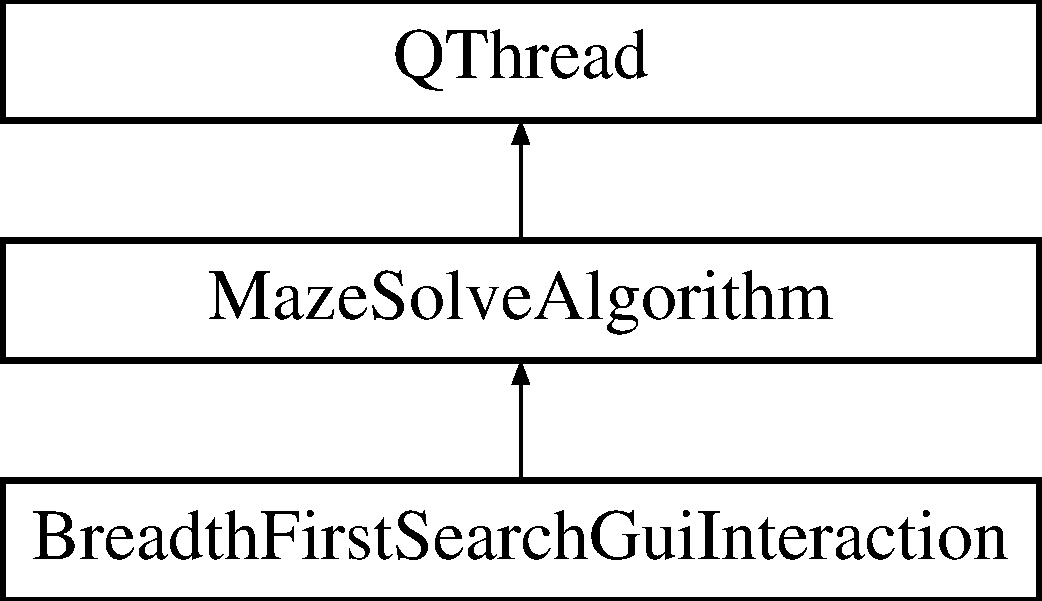
\includegraphics[height=3.000000cm]{class_breadth_first_search_gui_interaction}
\end{center}
\end{figure}
\subsection*{Public Member Functions}
\begin{DoxyCompactItemize}
\item 
\hyperlink{class_breadth_first_search_gui_interaction_a32769d981f2a07be1608288bfdb96efc}{Breadth\-First\-Search\-Gui\-Interaction} (\hyperlink{class_maze}{Maze} $\ast$maze)
\item 
\hyperlink{class_breadth_first_search_gui_interaction_a0277493bfd3ce130c0e95b3d841d8f9c}{$\sim$\-Breadth\-First\-Search\-Gui\-Interaction} ()
\item 
bool \hyperlink{class_breadth_first_search_gui_interaction_ad76cbe94351cb0d25fcf5d43468074e4}{solve} (int \&steps)
\end{DoxyCompactItemize}
\subsection*{Additional Inherited Members}


\subsection{Detailed Description}
Wraps logic of Breath\-First\-Search into class extending \hyperlink{class_maze_solve_algorithm}{Maze\-Solve\-Algorithm}. 

\subsection{Constructor \& Destructor Documentation}
\hypertarget{class_breadth_first_search_gui_interaction_a32769d981f2a07be1608288bfdb96efc}{\index{Breadth\-First\-Search\-Gui\-Interaction@{Breadth\-First\-Search\-Gui\-Interaction}!Breadth\-First\-Search\-Gui\-Interaction@{Breadth\-First\-Search\-Gui\-Interaction}}
\index{Breadth\-First\-Search\-Gui\-Interaction@{Breadth\-First\-Search\-Gui\-Interaction}!BreadthFirstSearchGuiInteraction@{Breadth\-First\-Search\-Gui\-Interaction}}
\subsubsection[{Breadth\-First\-Search\-Gui\-Interaction}]{\setlength{\rightskip}{0pt plus 5cm}Breadth\-First\-Search\-Gui\-Interaction\-::\-Breadth\-First\-Search\-Gui\-Interaction (
\begin{DoxyParamCaption}
\item[{{\bf Maze} $\ast$}]{maze}
\end{DoxyParamCaption}
)\hspace{0.3cm}{\ttfamily [inline]}}}\label{class_breadth_first_search_gui_interaction_a32769d981f2a07be1608288bfdb96efc}
Initializes both the breadth first search logic and its gui-\/representation. 
\begin{DoxyParams}{Parameters}
{\em maze} & \hyperlink{class_maze}{Maze} to be solved. \\
\hline
\end{DoxyParams}
\hypertarget{class_breadth_first_search_gui_interaction_a0277493bfd3ce130c0e95b3d841d8f9c}{\index{Breadth\-First\-Search\-Gui\-Interaction@{Breadth\-First\-Search\-Gui\-Interaction}!$\sim$\-Breadth\-First\-Search\-Gui\-Interaction@{$\sim$\-Breadth\-First\-Search\-Gui\-Interaction}}
\index{$\sim$\-Breadth\-First\-Search\-Gui\-Interaction@{$\sim$\-Breadth\-First\-Search\-Gui\-Interaction}!BreadthFirstSearchGuiInteraction@{Breadth\-First\-Search\-Gui\-Interaction}}
\subsubsection[{$\sim$\-Breadth\-First\-Search\-Gui\-Interaction}]{\setlength{\rightskip}{0pt plus 5cm}Breadth\-First\-Search\-Gui\-Interaction\-::$\sim$\-Breadth\-First\-Search\-Gui\-Interaction (
\begin{DoxyParamCaption}
{}
\end{DoxyParamCaption}
)\hspace{0.3cm}{\ttfamily [inline]}}}\label{class_breadth_first_search_gui_interaction_a0277493bfd3ce130c0e95b3d841d8f9c}
Deletes all objects associated to the algorithm and its gui representation from the heap. 

\subsection{Member Function Documentation}
\hypertarget{class_breadth_first_search_gui_interaction_ad76cbe94351cb0d25fcf5d43468074e4}{\index{Breadth\-First\-Search\-Gui\-Interaction@{Breadth\-First\-Search\-Gui\-Interaction}!solve@{solve}}
\index{solve@{solve}!BreadthFirstSearchGuiInteraction@{Breadth\-First\-Search\-Gui\-Interaction}}
\subsubsection[{solve}]{\setlength{\rightskip}{0pt plus 5cm}bool Breadth\-First\-Search\-Gui\-Interaction\-::solve (
\begin{DoxyParamCaption}
\item[{int \&}]{steps}
\end{DoxyParamCaption}
)\hspace{0.3cm}{\ttfamily [virtual]}}}\label{class_breadth_first_search_gui_interaction_ad76cbe94351cb0d25fcf5d43468074e4}
Starts solving the maze. 
\begin{DoxyParams}{Parameters}
{\em steps} & Fields visited till termination of the algorithm. \\
\hline
\end{DoxyParams}
\begin{DoxyReturn}{Returns}
True if the maze have been solved. False if not. 
\end{DoxyReturn}


Implements \hyperlink{class_maze_solve_algorithm_a3f957367c4afe52d29b0021766a478be}{Maze\-Solve\-Algorithm}.



The documentation for this class was generated from the following files\-:\begin{DoxyCompactItemize}
\item 
/home/travis/build/algdat/blatt-\/2-\/maze/src/ss17/algodat/maze/control/shortest\-\_\-path/breadth\-\_\-first\-\_\-search/\hyperlink{_breadth_first_search_gui_interaction_8h}{Breadth\-First\-Search\-Gui\-Interaction.\-h}\item 
/home/travis/build/algdat/blatt-\/2-\/maze/src/ss17/algodat/maze/control/shortest\-\_\-path/breadth\-\_\-first\-\_\-search/\hyperlink{_breadth_first_search_gui_interaction_8cpp}{Breadth\-First\-Search\-Gui\-Interaction.\-cpp}\end{DoxyCompactItemize}

\hypertarget{class_maze}{\section{Maze Class Reference}
\label{class_maze}\index{Maze@{Maze}}
}


The \hyperlink{class_maze}{Maze} class contains the model of the maze with functions to set an get fields of the maze.  




{\ttfamily \#include $<$maze.\-h$>$}

\subsection*{Public Types}
\begin{DoxyCompactItemize}
\item 
enum \hyperlink{class_maze_a7a19b706242876f2c597033b3374e7fa}{Maze\-Symbols} \{ \\*
\hyperlink{class_maze_a7a19b706242876f2c597033b3374e7faa4b3509571b07cde9b535f8358157d676}{Wall} =0, 
\hyperlink{class_maze_a7a19b706242876f2c597033b3374e7faac7cbc8392fac9738ef3dac458865d3eb}{Way}, 
\hyperlink{class_maze_a7a19b706242876f2c597033b3374e7faaf68b987d7cff7378d76e7b4159aeea6d}{Start}, 
\hyperlink{class_maze_a7a19b706242876f2c597033b3374e7faa752d570bd64e08ce1c7f358dd3cc6969}{End}, 
\\*
\hyperlink{class_maze_a7a19b706242876f2c597033b3374e7faaa87a698c7829b0c1f1b89cc93a44f2bc}{Result}
 \}
\end{DoxyCompactItemize}
\subsection*{Public Member Functions}
\begin{DoxyCompactItemize}
\item 
\hyperlink{class_maze_a1caad1867d6d3fa28fd3886272b2f618}{Maze} (const int width, const int height)
\begin{DoxyCompactList}\small\item\em \hyperlink{class_maze_a1caad1867d6d3fa28fd3886272b2f618}{Maze\-::\-Maze} initializes the maze. \end{DoxyCompactList}\item 
\hyperlink{class_maze_a4f187353f595193318ac66133a22287e}{$\sim$\-Maze} ()
\begin{DoxyCompactList}\small\item\em \hyperlink{class_maze_a4f187353f595193318ac66133a22287e}{Maze\-::$\sim$\-Maze} deletes the mazearray on the heap. \end{DoxyCompactList}\item 
void \hyperlink{class_maze_a2d05ee06d2d4b6b9abe001e77a256c70}{set\-Maze\-Field} (const int \&pos\-Width, const int \&pos\-Height, \hyperlink{class_maze_a7a19b706242876f2c597033b3374e7fa}{Maze\-Symbols} value)
\begin{DoxyCompactList}\small\item\em \hyperlink{class_maze_a2d05ee06d2d4b6b9abe001e77a256c70}{Maze\-::set\-Maze\-Field} sets a field of the maze. \end{DoxyCompactList}\item 
int \hyperlink{class_maze_ac0fa84d55a0bf27854b1f8a7f0d7cebc}{get\-Maze\-Field} (const int \&pos\-Width, const int \&pos\-Height)
\begin{DoxyCompactList}\small\item\em \hyperlink{class_maze_ac0fa84d55a0bf27854b1f8a7f0d7cebc}{Maze\-::get\-Maze\-Field} returns the field on the deleivered position. \end{DoxyCompactList}\item 
int \hyperlink{class_maze_a55deabec3636694a2658ff902fe83a9b}{get\-Width} () const 
\begin{DoxyCompactList}\small\item\em \hyperlink{class_maze_a55deabec3636694a2658ff902fe83a9b}{Maze\-::get\-Width} getter for m\-\_\-width. \end{DoxyCompactList}\item 
int \hyperlink{class_maze_a3cfe8e5f193ff2ed9d6915c8841d376a}{get\-Height} () const 
\begin{DoxyCompactList}\small\item\em \hyperlink{class_maze_a3cfe8e5f193ff2ed9d6915c8841d376a}{Maze\-::get\-Height} setter for m\-\_\-height. \end{DoxyCompactList}\end{DoxyCompactItemize}


\subsection{Detailed Description}
The \hyperlink{class_maze}{Maze} class contains the model of the maze with functions to set an get fields of the maze. 

\subsection{Member Enumeration Documentation}
\hypertarget{class_maze_a7a19b706242876f2c597033b3374e7fa}{\index{Maze@{Maze}!Maze\-Symbols@{Maze\-Symbols}}
\index{Maze\-Symbols@{Maze\-Symbols}!Maze@{Maze}}
\subsubsection[{Maze\-Symbols}]{\setlength{\rightskip}{0pt plus 5cm}enum {\bf Maze\-::\-Maze\-Symbols}}}\label{class_maze_a7a19b706242876f2c597033b3374e7fa}
\begin{Desc}
\item[Enumerator]\par
\begin{description}
\index{Wall@{Wall}!Maze@{Maze}}\index{Maze@{Maze}!Wall@{Wall}}\item[{\em 
\hypertarget{class_maze_a7a19b706242876f2c597033b3374e7faa4b3509571b07cde9b535f8358157d676}{Wall}\label{class_maze_a7a19b706242876f2c597033b3374e7faa4b3509571b07cde9b535f8358157d676}
}]\index{Way@{Way}!Maze@{Maze}}\index{Maze@{Maze}!Way@{Way}}\item[{\em 
\hypertarget{class_maze_a7a19b706242876f2c597033b3374e7faac7cbc8392fac9738ef3dac458865d3eb}{Way}\label{class_maze_a7a19b706242876f2c597033b3374e7faac7cbc8392fac9738ef3dac458865d3eb}
}]\index{Start@{Start}!Maze@{Maze}}\index{Maze@{Maze}!Start@{Start}}\item[{\em 
\hypertarget{class_maze_a7a19b706242876f2c597033b3374e7faaf68b987d7cff7378d76e7b4159aeea6d}{Start}\label{class_maze_a7a19b706242876f2c597033b3374e7faaf68b987d7cff7378d76e7b4159aeea6d}
}]\index{End@{End}!Maze@{Maze}}\index{Maze@{Maze}!End@{End}}\item[{\em 
\hypertarget{class_maze_a7a19b706242876f2c597033b3374e7faa752d570bd64e08ce1c7f358dd3cc6969}{End}\label{class_maze_a7a19b706242876f2c597033b3374e7faa752d570bd64e08ce1c7f358dd3cc6969}
}]\index{Result@{Result}!Maze@{Maze}}\index{Maze@{Maze}!Result@{Result}}\item[{\em 
\hypertarget{class_maze_a7a19b706242876f2c597033b3374e7faaa87a698c7829b0c1f1b89cc93a44f2bc}{Result}\label{class_maze_a7a19b706242876f2c597033b3374e7faaa87a698c7829b0c1f1b89cc93a44f2bc}
}]\end{description}
\end{Desc}


\subsection{Constructor \& Destructor Documentation}
\hypertarget{class_maze_a1caad1867d6d3fa28fd3886272b2f618}{\index{Maze@{Maze}!Maze@{Maze}}
\index{Maze@{Maze}!Maze@{Maze}}
\subsubsection[{Maze}]{\setlength{\rightskip}{0pt plus 5cm}Maze\-::\-Maze (
\begin{DoxyParamCaption}
\item[{const int}]{width, }
\item[{const int}]{height}
\end{DoxyParamCaption}
)}}\label{class_maze_a1caad1867d6d3fa28fd3886272b2f618}


\hyperlink{class_maze_a1caad1867d6d3fa28fd3886272b2f618}{Maze\-::\-Maze} initializes the maze. 


\begin{DoxyParams}{Parameters}
{\em width} & width of the maze \\
\hline
{\em height} & height of the maze \\
\hline
\end{DoxyParams}
\hypertarget{class_maze_a4f187353f595193318ac66133a22287e}{\index{Maze@{Maze}!$\sim$\-Maze@{$\sim$\-Maze}}
\index{$\sim$\-Maze@{$\sim$\-Maze}!Maze@{Maze}}
\subsubsection[{$\sim$\-Maze}]{\setlength{\rightskip}{0pt plus 5cm}Maze\-::$\sim$\-Maze (
\begin{DoxyParamCaption}
{}
\end{DoxyParamCaption}
)}}\label{class_maze_a4f187353f595193318ac66133a22287e}


\hyperlink{class_maze_a4f187353f595193318ac66133a22287e}{Maze\-::$\sim$\-Maze} deletes the mazearray on the heap. 



\subsection{Member Function Documentation}
\hypertarget{class_maze_a3cfe8e5f193ff2ed9d6915c8841d376a}{\index{Maze@{Maze}!get\-Height@{get\-Height}}
\index{get\-Height@{get\-Height}!Maze@{Maze}}
\subsubsection[{get\-Height}]{\setlength{\rightskip}{0pt plus 5cm}int Maze\-::get\-Height (
\begin{DoxyParamCaption}
{}
\end{DoxyParamCaption}
) const}}\label{class_maze_a3cfe8e5f193ff2ed9d6915c8841d376a}


\hyperlink{class_maze_a3cfe8e5f193ff2ed9d6915c8841d376a}{Maze\-::get\-Height} setter for m\-\_\-height. 

\begin{DoxyReturn}{Returns}
height 
\end{DoxyReturn}
\hypertarget{class_maze_ac0fa84d55a0bf27854b1f8a7f0d7cebc}{\index{Maze@{Maze}!get\-Maze\-Field@{get\-Maze\-Field}}
\index{get\-Maze\-Field@{get\-Maze\-Field}!Maze@{Maze}}
\subsubsection[{get\-Maze\-Field}]{\setlength{\rightskip}{0pt plus 5cm}int Maze\-::get\-Maze\-Field (
\begin{DoxyParamCaption}
\item[{const int \&}]{pos\-Width, }
\item[{const int \&}]{height}
\end{DoxyParamCaption}
)}}\label{class_maze_ac0fa84d55a0bf27854b1f8a7f0d7cebc}


\hyperlink{class_maze_ac0fa84d55a0bf27854b1f8a7f0d7cebc}{Maze\-::get\-Maze\-Field} returns the field on the deleivered position. 


\begin{DoxyParams}{Parameters}
{\em pos\-Width} & the x-\/position \\
\hline
{\em height} & the y-\/position \\
\hline
\end{DoxyParams}
\begin{DoxyReturn}{Returns}
the value on the selected field 
\end{DoxyReturn}
\hypertarget{class_maze_a55deabec3636694a2658ff902fe83a9b}{\index{Maze@{Maze}!get\-Width@{get\-Width}}
\index{get\-Width@{get\-Width}!Maze@{Maze}}
\subsubsection[{get\-Width}]{\setlength{\rightskip}{0pt plus 5cm}int Maze\-::get\-Width (
\begin{DoxyParamCaption}
{}
\end{DoxyParamCaption}
) const}}\label{class_maze_a55deabec3636694a2658ff902fe83a9b}


\hyperlink{class_maze_a55deabec3636694a2658ff902fe83a9b}{Maze\-::get\-Width} getter for m\-\_\-width. 

\begin{DoxyReturn}{Returns}
width 
\end{DoxyReturn}
\hypertarget{class_maze_a2d05ee06d2d4b6b9abe001e77a256c70}{\index{Maze@{Maze}!set\-Maze\-Field@{set\-Maze\-Field}}
\index{set\-Maze\-Field@{set\-Maze\-Field}!Maze@{Maze}}
\subsubsection[{set\-Maze\-Field}]{\setlength{\rightskip}{0pt plus 5cm}void Maze\-::set\-Maze\-Field (
\begin{DoxyParamCaption}
\item[{const int \&}]{pos\-Width, }
\item[{const int \&}]{pos\-Height, }
\item[{{\bf Maze\-Symbols}}]{value}
\end{DoxyParamCaption}
)}}\label{class_maze_a2d05ee06d2d4b6b9abe001e77a256c70}


\hyperlink{class_maze_a2d05ee06d2d4b6b9abe001e77a256c70}{Maze\-::set\-Maze\-Field} sets a field of the maze. 


\begin{DoxyParams}{Parameters}
{\em pos\-Width} & the x-\/position of the element \\
\hline
{\em pos\-Height} & the y-\/position of the element \\
\hline
{\em value} & \\
\hline
\end{DoxyParams}


The documentation for this class was generated from the following files\-:\begin{DoxyCompactItemize}
\item 
/home/travis/build/algdat/blatt-\/2-\/maze/src/ss17/algodat/maze/model/\hyperlink{maze_8h}{maze.\-h}\item 
/home/travis/build/algdat/blatt-\/2-\/maze/src/ss17/algodat/maze/model/\hyperlink{maze_8cpp}{maze.\-cpp}\end{DoxyCompactItemize}

\hypertarget{class_maze_generator}{\section{Maze\-Generator Class Reference}
\label{class_maze_generator}\index{Maze\-Generator@{Maze\-Generator}}
}


{\ttfamily \#include $<$mazegenerator.\-h$>$}

\subsection*{Public Member Functions}
\begin{DoxyCompactItemize}
\item 
\hyperlink{class_maze_generator_ad2614d8adc80721dbae5660402d48573}{Maze\-Generator} ()
\end{DoxyCompactItemize}
\subsection*{Static Public Member Functions}
\begin{DoxyCompactItemize}
\item 
static \hyperlink{class_maze}{Maze} $\ast$ \hyperlink{class_maze_generator_ad4be0b35657e25065168e1d6fcebfb8d}{generate\-Maze} (const int width, const int hight)
\end{DoxyCompactItemize}


\subsection{Constructor \& Destructor Documentation}
\hypertarget{class_maze_generator_ad2614d8adc80721dbae5660402d48573}{\index{Maze\-Generator@{Maze\-Generator}!Maze\-Generator@{Maze\-Generator}}
\index{Maze\-Generator@{Maze\-Generator}!MazeGenerator@{Maze\-Generator}}
\subsubsection[{Maze\-Generator}]{\setlength{\rightskip}{0pt plus 5cm}Maze\-Generator\-::\-Maze\-Generator (
\begin{DoxyParamCaption}
{}
\end{DoxyParamCaption}
)}}\label{class_maze_generator_ad2614d8adc80721dbae5660402d48573}


\subsection{Member Function Documentation}
\hypertarget{class_maze_generator_ad4be0b35657e25065168e1d6fcebfb8d}{\index{Maze\-Generator@{Maze\-Generator}!generate\-Maze@{generate\-Maze}}
\index{generate\-Maze@{generate\-Maze}!MazeGenerator@{Maze\-Generator}}
\subsubsection[{generate\-Maze}]{\setlength{\rightskip}{0pt plus 5cm}{\bf Maze} $\ast$ Maze\-Generator\-::generate\-Maze (
\begin{DoxyParamCaption}
\item[{const int}]{width, }
\item[{const int}]{hight}
\end{DoxyParamCaption}
)\hspace{0.3cm}{\ttfamily [static]}}}\label{class_maze_generator_ad4be0b35657e25065168e1d6fcebfb8d}


The documentation for this class was generated from the following files\-:\begin{DoxyCompactItemize}
\item 
/home/travis/build/algdat/blatt-\/2-\/maze/src/ss17/algodat/maze/control/\hyperlink{mazegenerator_8h}{mazegenerator.\-h}\item 
/home/travis/build/algdat/blatt-\/2-\/maze/src/ss17/algodat/maze/control/\hyperlink{mazegenerator_8cpp}{mazegenerator.\-cpp}\end{DoxyCompactItemize}

\hypertarget{class_maze_gui}{\section{Maze\-Gui Class Reference}
\label{class_maze_gui}\index{Maze\-Gui@{Maze\-Gui}}
}


{\ttfamily \#include $<$mazegui.\-h$>$}

Inheritance diagram for Maze\-Gui\-:\begin{figure}[H]
\begin{center}
\leavevmode
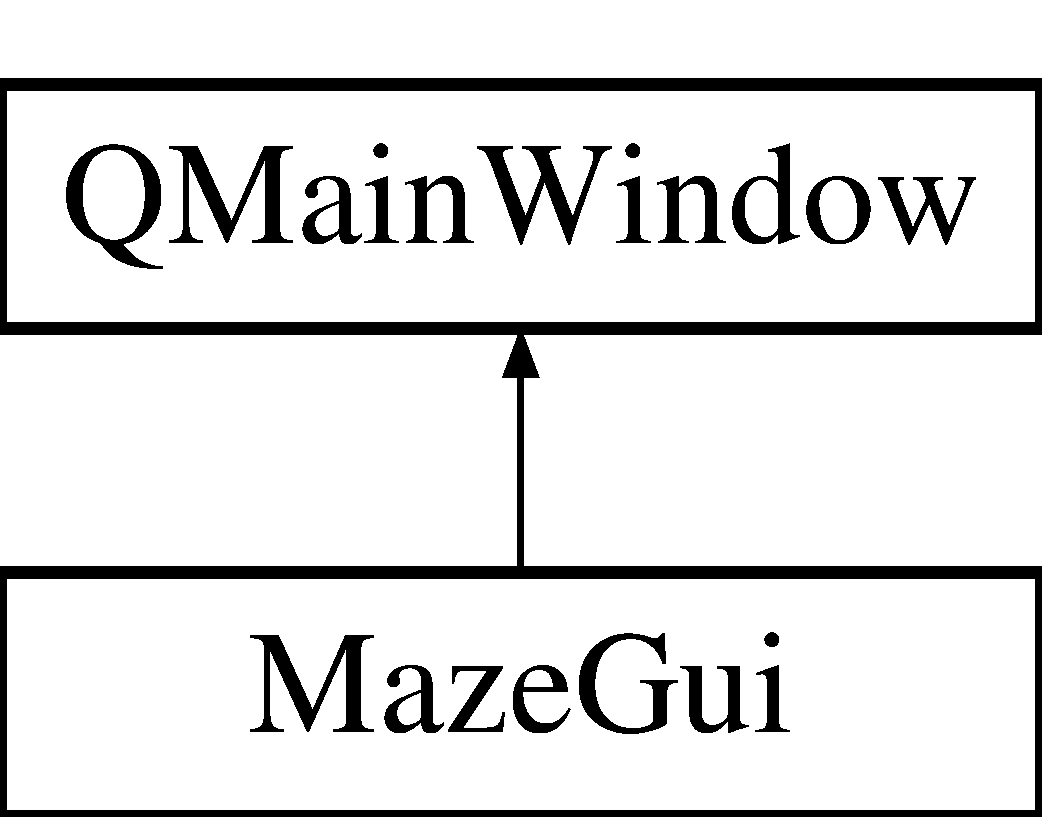
\includegraphics[height=2.000000cm]{class_maze_gui}
\end{center}
\end{figure}
\subsection*{Public Slots}
\begin{DoxyCompactItemize}
\item 
void \hyperlink{class_maze_gui_aa3b128bc77c97364bd0abcfab50facac}{start\-Algorithm} ()
\begin{DoxyCompactList}\small\item\em \hyperlink{class_maze_gui_aa3b128bc77c97364bd0abcfab50facac}{Maze\-Gui\-::start\-Algorithm} starts the algorithm choosen in the combo box, measures the time, sets the display for steps and the elapsed time. \end{DoxyCompactList}\item 
void \hyperlink{class_maze_gui_a951cf062b683fc7b9e35f5e655b0f609}{generate\-Maze} ()
\begin{DoxyCompactList}\small\item\em \hyperlink{class_maze_gui_a951cf062b683fc7b9e35f5e655b0f609}{Maze\-Gui\-::generate\-Maze} Generates a random maze. \end{DoxyCompactList}\item 
void \hyperlink{class_maze_gui_ad16d7a5be838ffbde722bfdeb05859a4}{update\-Maze\-Slot} ()
\item 
void \hyperlink{class_maze_gui_a11530ab74ba41b8013ecacc25aca3363}{update\-L\-C\-D\-Displays\-Slot} ()
\end{DoxyCompactItemize}
\subsection*{Public Member Functions}
\begin{DoxyCompactItemize}
\item 
\hyperlink{class_maze_gui_aea46561b3539431d4c71515cb50ec530}{Maze\-Gui} (Q\-Widget $\ast$parent=0)
\begin{DoxyCompactList}\small\item\em \hyperlink{class_maze_gui_aea46561b3539431d4c71515cb50ec530}{Maze\-Gui\-::\-Maze\-Gui} constructor sets up the gui such es the sockets and slots. \end{DoxyCompactList}\item 
\hyperlink{class_maze_gui_af230996793f8246cd6f50f5c69ac2a79}{$\sim$\-Maze\-Gui} ()
\begin{DoxyCompactList}\small\item\em \hyperlink{class_maze_gui_af230996793f8246cd6f50f5c69ac2a79}{Maze\-Gui\-::$\sim$\-Maze\-Gui} delets all heap elements. \end{DoxyCompactList}\item 
void \hyperlink{class_maze_gui_a5bcc8fc361cc77fd741c690775bf5a04}{set\-Maze} (\hyperlink{class_maze}{Maze} $\ast$maze)
\begin{DoxyCompactList}\small\item\em \hyperlink{class_maze_gui_a5bcc8fc361cc77fd741c690775bf5a04}{Maze\-Gui\-::set\-Maze} Sets the maze. \end{DoxyCompactList}\item 
void \hyperlink{class_maze_gui_a42bc86307a9cfecf3f42084a0dabdfb3}{draw\-Empty\-Maze} ()
\begin{DoxyCompactList}\small\item\em Maze\-Gui\-::generate\-Field Generates a \hyperlink{class_maze}{Maze} whith the delivered width and height. \end{DoxyCompactList}\item 
void \hyperlink{class_maze_gui_ab6a12bf649ff8a9adf48696626f5c2a4}{draw\-Maze} ()
\begin{DoxyCompactList}\small\item\em \hyperlink{class_maze_gui_a5bcc8fc361cc77fd741c690775bf5a04}{Maze\-Gui\-::set\-Maze} Gets an two dimensional Array which has the size of the field and contains a colorcode for every field. The colores where set and printed. \end{DoxyCompactList}\end{DoxyCompactItemize}


\subsection{Constructor \& Destructor Documentation}
\hypertarget{class_maze_gui_aea46561b3539431d4c71515cb50ec530}{\index{Maze\-Gui@{Maze\-Gui}!Maze\-Gui@{Maze\-Gui}}
\index{Maze\-Gui@{Maze\-Gui}!MazeGui@{Maze\-Gui}}
\subsubsection[{Maze\-Gui}]{\setlength{\rightskip}{0pt plus 5cm}Maze\-Gui\-::\-Maze\-Gui (
\begin{DoxyParamCaption}
\item[{Q\-Widget $\ast$}]{parent = {\ttfamily 0}}
\end{DoxyParamCaption}
)\hspace{0.3cm}{\ttfamily [explicit]}}}\label{class_maze_gui_aea46561b3539431d4c71515cb50ec530}


\hyperlink{class_maze_gui_aea46561b3539431d4c71515cb50ec530}{Maze\-Gui\-::\-Maze\-Gui} constructor sets up the gui such es the sockets and slots. 


\begin{DoxyParams}{Parameters}
{\em parent} & \\
\hline
\end{DoxyParams}
\hypertarget{class_maze_gui_af230996793f8246cd6f50f5c69ac2a79}{\index{Maze\-Gui@{Maze\-Gui}!$\sim$\-Maze\-Gui@{$\sim$\-Maze\-Gui}}
\index{$\sim$\-Maze\-Gui@{$\sim$\-Maze\-Gui}!MazeGui@{Maze\-Gui}}
\subsubsection[{$\sim$\-Maze\-Gui}]{\setlength{\rightskip}{0pt plus 5cm}Maze\-Gui\-::$\sim$\-Maze\-Gui (
\begin{DoxyParamCaption}
{}
\end{DoxyParamCaption}
)}}\label{class_maze_gui_af230996793f8246cd6f50f5c69ac2a79}


\hyperlink{class_maze_gui_af230996793f8246cd6f50f5c69ac2a79}{Maze\-Gui\-::$\sim$\-Maze\-Gui} delets all heap elements. 



\subsection{Member Function Documentation}
\hypertarget{class_maze_gui_a42bc86307a9cfecf3f42084a0dabdfb3}{\index{Maze\-Gui@{Maze\-Gui}!draw\-Empty\-Maze@{draw\-Empty\-Maze}}
\index{draw\-Empty\-Maze@{draw\-Empty\-Maze}!MazeGui@{Maze\-Gui}}
\subsubsection[{draw\-Empty\-Maze}]{\setlength{\rightskip}{0pt plus 5cm}void Maze\-Gui\-::draw\-Empty\-Maze (
\begin{DoxyParamCaption}
{}
\end{DoxyParamCaption}
)}}\label{class_maze_gui_a42bc86307a9cfecf3f42084a0dabdfb3}


Maze\-Gui\-::generate\-Field Generates a \hyperlink{class_maze}{Maze} whith the delivered width and height. 


\begin{DoxyParams}{Parameters}
{\em width} & \\
\hline
{\em height} & \\
\hline
\end{DoxyParams}
\hypertarget{class_maze_gui_ab6a12bf649ff8a9adf48696626f5c2a4}{\index{Maze\-Gui@{Maze\-Gui}!draw\-Maze@{draw\-Maze}}
\index{draw\-Maze@{draw\-Maze}!MazeGui@{Maze\-Gui}}
\subsubsection[{draw\-Maze}]{\setlength{\rightskip}{0pt plus 5cm}void Maze\-Gui\-::draw\-Maze (
\begin{DoxyParamCaption}
{}
\end{DoxyParamCaption}
)}}\label{class_maze_gui_ab6a12bf649ff8a9adf48696626f5c2a4}


\hyperlink{class_maze_gui_a5bcc8fc361cc77fd741c690775bf5a04}{Maze\-Gui\-::set\-Maze} Gets an two dimensional Array which has the size of the field and contains a colorcode for every field. The colores where set and printed. 


\begin{DoxyParams}{Parameters}
{\em field} & maze field \\
\hline
{\em width} & the width of the maze \\
\hline
{\em height} & the height of the maze \\
\hline
\end{DoxyParams}
\hypertarget{class_maze_gui_a951cf062b683fc7b9e35f5e655b0f609}{\index{Maze\-Gui@{Maze\-Gui}!generate\-Maze@{generate\-Maze}}
\index{generate\-Maze@{generate\-Maze}!MazeGui@{Maze\-Gui}}
\subsubsection[{generate\-Maze}]{\setlength{\rightskip}{0pt plus 5cm}void Maze\-Gui\-::generate\-Maze (
\begin{DoxyParamCaption}
{}
\end{DoxyParamCaption}
)\hspace{0.3cm}{\ttfamily [slot]}}}\label{class_maze_gui_a951cf062b683fc7b9e35f5e655b0f609}


\hyperlink{class_maze_gui_a951cf062b683fc7b9e35f5e655b0f609}{Maze\-Gui\-::generate\-Maze} Generates a random maze. 


\begin{DoxyParams}{Parameters}
{\em maze} & array which contains all maze values \\
\hline
{\em width} & width of the maze \\
\hline
{\em height} & height of the maze \\
\hline
\end{DoxyParams}
\begin{DoxyReturn}{Returns}
error code (0 if successful) 
\end{DoxyReturn}
\hypertarget{class_maze_gui_a5bcc8fc361cc77fd741c690775bf5a04}{\index{Maze\-Gui@{Maze\-Gui}!set\-Maze@{set\-Maze}}
\index{set\-Maze@{set\-Maze}!MazeGui@{Maze\-Gui}}
\subsubsection[{set\-Maze}]{\setlength{\rightskip}{0pt plus 5cm}void Maze\-Gui\-::set\-Maze (
\begin{DoxyParamCaption}
\item[{{\bf Maze} $\ast$}]{maze}
\end{DoxyParamCaption}
)}}\label{class_maze_gui_a5bcc8fc361cc77fd741c690775bf5a04}


\hyperlink{class_maze_gui_a5bcc8fc361cc77fd741c690775bf5a04}{Maze\-Gui\-::set\-Maze} Sets the maze. 

\hypertarget{class_maze_gui_aa3b128bc77c97364bd0abcfab50facac}{\index{Maze\-Gui@{Maze\-Gui}!start\-Algorithm@{start\-Algorithm}}
\index{start\-Algorithm@{start\-Algorithm}!MazeGui@{Maze\-Gui}}
\subsubsection[{start\-Algorithm}]{\setlength{\rightskip}{0pt plus 5cm}void Maze\-Gui\-::start\-Algorithm (
\begin{DoxyParamCaption}
{}
\end{DoxyParamCaption}
)\hspace{0.3cm}{\ttfamily [slot]}}}\label{class_maze_gui_aa3b128bc77c97364bd0abcfab50facac}


\hyperlink{class_maze_gui_aa3b128bc77c97364bd0abcfab50facac}{Maze\-Gui\-::start\-Algorithm} starts the algorithm choosen in the combo box, measures the time, sets the display for steps and the elapsed time. 

\hypertarget{class_maze_gui_a11530ab74ba41b8013ecacc25aca3363}{\index{Maze\-Gui@{Maze\-Gui}!update\-L\-C\-D\-Displays\-Slot@{update\-L\-C\-D\-Displays\-Slot}}
\index{update\-L\-C\-D\-Displays\-Slot@{update\-L\-C\-D\-Displays\-Slot}!MazeGui@{Maze\-Gui}}
\subsubsection[{update\-L\-C\-D\-Displays\-Slot}]{\setlength{\rightskip}{0pt plus 5cm}void Maze\-Gui\-::update\-L\-C\-D\-Displays\-Slot (
\begin{DoxyParamCaption}
{}
\end{DoxyParamCaption}
)\hspace{0.3cm}{\ttfamily [slot]}}}\label{class_maze_gui_a11530ab74ba41b8013ecacc25aca3363}
\hypertarget{class_maze_gui_ad16d7a5be838ffbde722bfdeb05859a4}{\index{Maze\-Gui@{Maze\-Gui}!update\-Maze\-Slot@{update\-Maze\-Slot}}
\index{update\-Maze\-Slot@{update\-Maze\-Slot}!MazeGui@{Maze\-Gui}}
\subsubsection[{update\-Maze\-Slot}]{\setlength{\rightskip}{0pt plus 5cm}void Maze\-Gui\-::update\-Maze\-Slot (
\begin{DoxyParamCaption}
{}
\end{DoxyParamCaption}
)\hspace{0.3cm}{\ttfamily [slot]}}}\label{class_maze_gui_ad16d7a5be838ffbde722bfdeb05859a4}


The documentation for this class was generated from the following files\-:\begin{DoxyCompactItemize}
\item 
/home/travis/build/algdat/blatt-\/2-\/maze/src/ss17/algodat/maze/view/\hyperlink{mazegui_8h}{mazegui.\-h}\item 
/home/travis/build/algdat/blatt-\/2-\/maze/src/ss17/algodat/maze/view/\hyperlink{mazegui_8cpp}{mazegui.\-cpp}\end{DoxyCompactItemize}

\hypertarget{class_maze_solve_algorithm}{\section{Maze\-Solve\-Algorithm Class Reference}
\label{class_maze_solve_algorithm}\index{Maze\-Solve\-Algorithm@{Maze\-Solve\-Algorithm}}
}


The Maze\-Algorithm class Baseclass have to be derived by all maze solve algorithm classes contains the datastructures for the maze such as methods to redrow.  




{\ttfamily \#include $<$mazealgorithm.\-h$>$}

Inheritance diagram for Maze\-Solve\-Algorithm\-:\begin{figure}[H]
\begin{center}
\leavevmode
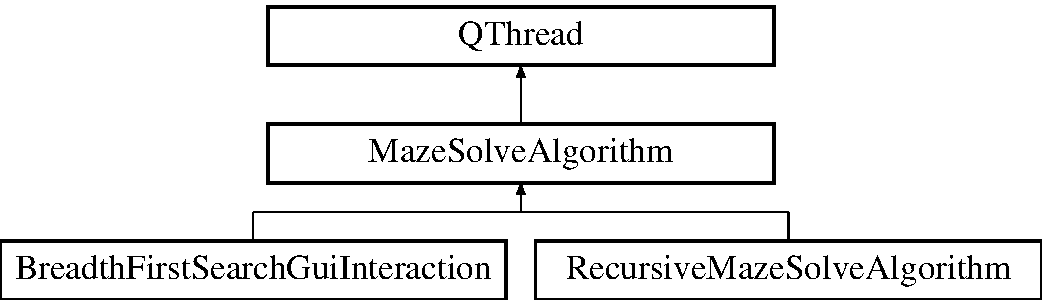
\includegraphics[height=3.000000cm]{class_maze_solve_algorithm}
\end{center}
\end{figure}
\subsection*{Signals}
\begin{DoxyCompactItemize}
\item 
void \hyperlink{class_maze_solve_algorithm_ad2903ca429a66b0f7558e169ff2c47c3}{redraw} ()
\item 
void \hyperlink{class_maze_solve_algorithm_abe3dc4ab4896e39d9ce9bc34138bb138}{signal\-L\-C\-D\-Displays} ()
\end{DoxyCompactItemize}
\subsection*{Public Member Functions}
\begin{DoxyCompactItemize}
\item 
\hyperlink{class_maze_solve_algorithm_a403d0adac396c5aad4500e8700b0309d}{Maze\-Solve\-Algorithm} (\hyperlink{class_maze}{Maze} $\ast$maze)
\begin{DoxyCompactList}\small\item\em \hyperlink{class_maze_solve_algorithm_a403d0adac396c5aad4500e8700b0309d}{Maze\-Solve\-Algorithm\-::\-Maze\-Solve\-Algorithm} sets the maze and initializes all variables. \end{DoxyCompactList}\item 
int \hyperlink{class_maze_solve_algorithm_a69f1c6da39848354f26a5d6fb7dce3f6}{get\-Steps} () const 
\begin{DoxyCompactList}\small\item\em \hyperlink{class_maze_solve_algorithm_a69f1c6da39848354f26a5d6fb7dce3f6}{Maze\-Solve\-Algorithm\-::get\-Steps} getter for m\-\_\-steps. \end{DoxyCompactList}\item 
double \hyperlink{class_maze_solve_algorithm_a9522bc9a8fb6760e5bec78bfcc52ef53}{get\-Elapsed\-Time} () const 
\begin{DoxyCompactList}\small\item\em \hyperlink{class_maze_solve_algorithm_a9522bc9a8fb6760e5bec78bfcc52ef53}{Maze\-Solve\-Algorithm\-::get\-Elapsed\-Time} getter for m\-\_\-elapsed\-Time. \end{DoxyCompactList}\item 
bool \hyperlink{class_maze_solve_algorithm_ad1b31dffa81ae7ee84fd511aadc0fdb8}{is\-Solved} () const 
\begin{DoxyCompactList}\small\item\em \hyperlink{class_maze_solve_algorithm_ad1b31dffa81ae7ee84fd511aadc0fdb8}{Maze\-Solve\-Algorithm\-::is\-Solved} getter for m\-\_\-is\-Solved. \end{DoxyCompactList}\end{DoxyCompactItemize}
\subsection*{Public Attributes}
\begin{DoxyCompactItemize}
\item 
\hyperlink{class_maze}{Maze} $\ast$ \hyperlink{class_maze_solve_algorithm_a22988c0e0a5eaea83ce360be8e3a9ebb}{m\-\_\-maze}
\item 
int \hyperlink{class_maze_solve_algorithm_a16f9e281c4bcdc47575d7b75c244652e}{m\-\_\-steps}
\item 
double \hyperlink{class_maze_solve_algorithm_a1ca82a6e1f52cdb2f6bc3ea7b332e2f2}{m\-\_\-elapsed\-Time}
\item 
bool \hyperlink{class_maze_solve_algorithm_a1c7f66e1bc5c91f9d007ba0a79d239d0}{m\-\_\-solved}
\end{DoxyCompactItemize}
\subsection*{Protected Member Functions}
\begin{DoxyCompactItemize}
\item 
void \hyperlink{class_maze_solve_algorithm_a3e545c01367136ed0a02d9bb6c2b3ede}{run} ()
\begin{DoxyCompactList}\small\item\em Maze\-Algorithm\-::run run method starts the solving algorithm such as the time measurement, signals the gui to display the values. \end{DoxyCompactList}\item 
virtual bool \hyperlink{class_maze_solve_algorithm_a3f957367c4afe52d29b0021766a478be}{solve} (int \&steps)=0
\end{DoxyCompactItemize}


\subsection{Detailed Description}
The Maze\-Algorithm class Baseclass have to be derived by all maze solve algorithm classes contains the datastructures for the maze such as methods to redrow. 

\subsection{Constructor \& Destructor Documentation}
\hypertarget{class_maze_solve_algorithm_a403d0adac396c5aad4500e8700b0309d}{\index{Maze\-Solve\-Algorithm@{Maze\-Solve\-Algorithm}!Maze\-Solve\-Algorithm@{Maze\-Solve\-Algorithm}}
\index{Maze\-Solve\-Algorithm@{Maze\-Solve\-Algorithm}!MazeSolveAlgorithm@{Maze\-Solve\-Algorithm}}
\subsubsection[{Maze\-Solve\-Algorithm}]{\setlength{\rightskip}{0pt plus 5cm}Maze\-Solve\-Algorithm\-::\-Maze\-Solve\-Algorithm (
\begin{DoxyParamCaption}
\item[{{\bf Maze} $\ast$}]{maze}
\end{DoxyParamCaption}
)}}\label{class_maze_solve_algorithm_a403d0adac396c5aad4500e8700b0309d}


\hyperlink{class_maze_solve_algorithm_a403d0adac396c5aad4500e8700b0309d}{Maze\-Solve\-Algorithm\-::\-Maze\-Solve\-Algorithm} sets the maze and initializes all variables. 


\begin{DoxyParams}{Parameters}
{\em maze} & \\
\hline
{\em width} & \\
\hline
{\em height} & \\
\hline
\end{DoxyParams}


\subsection{Member Function Documentation}
\hypertarget{class_maze_solve_algorithm_a9522bc9a8fb6760e5bec78bfcc52ef53}{\index{Maze\-Solve\-Algorithm@{Maze\-Solve\-Algorithm}!get\-Elapsed\-Time@{get\-Elapsed\-Time}}
\index{get\-Elapsed\-Time@{get\-Elapsed\-Time}!MazeSolveAlgorithm@{Maze\-Solve\-Algorithm}}
\subsubsection[{get\-Elapsed\-Time}]{\setlength{\rightskip}{0pt plus 5cm}double Maze\-Solve\-Algorithm\-::get\-Elapsed\-Time (
\begin{DoxyParamCaption}
{}
\end{DoxyParamCaption}
) const}}\label{class_maze_solve_algorithm_a9522bc9a8fb6760e5bec78bfcc52ef53}


\hyperlink{class_maze_solve_algorithm_a9522bc9a8fb6760e5bec78bfcc52ef53}{Maze\-Solve\-Algorithm\-::get\-Elapsed\-Time} getter for m\-\_\-elapsed\-Time. 

\begin{DoxyReturn}{Returns}
elapsed time 
\end{DoxyReturn}
\hypertarget{class_maze_solve_algorithm_a69f1c6da39848354f26a5d6fb7dce3f6}{\index{Maze\-Solve\-Algorithm@{Maze\-Solve\-Algorithm}!get\-Steps@{get\-Steps}}
\index{get\-Steps@{get\-Steps}!MazeSolveAlgorithm@{Maze\-Solve\-Algorithm}}
\subsubsection[{get\-Steps}]{\setlength{\rightskip}{0pt plus 5cm}int Maze\-Solve\-Algorithm\-::get\-Steps (
\begin{DoxyParamCaption}
{}
\end{DoxyParamCaption}
) const}}\label{class_maze_solve_algorithm_a69f1c6da39848354f26a5d6fb7dce3f6}


\hyperlink{class_maze_solve_algorithm_a69f1c6da39848354f26a5d6fb7dce3f6}{Maze\-Solve\-Algorithm\-::get\-Steps} getter for m\-\_\-steps. 

\begin{DoxyReturn}{Returns}
nr of steps 
\end{DoxyReturn}
\hypertarget{class_maze_solve_algorithm_ad1b31dffa81ae7ee84fd511aadc0fdb8}{\index{Maze\-Solve\-Algorithm@{Maze\-Solve\-Algorithm}!is\-Solved@{is\-Solved}}
\index{is\-Solved@{is\-Solved}!MazeSolveAlgorithm@{Maze\-Solve\-Algorithm}}
\subsubsection[{is\-Solved}]{\setlength{\rightskip}{0pt plus 5cm}bool Maze\-Solve\-Algorithm\-::is\-Solved (
\begin{DoxyParamCaption}
{}
\end{DoxyParamCaption}
) const}}\label{class_maze_solve_algorithm_ad1b31dffa81ae7ee84fd511aadc0fdb8}


\hyperlink{class_maze_solve_algorithm_ad1b31dffa81ae7ee84fd511aadc0fdb8}{Maze\-Solve\-Algorithm\-::is\-Solved} getter for m\-\_\-is\-Solved. 

\begin{DoxyReturn}{Returns}
solved flag 
\end{DoxyReturn}
\hypertarget{class_maze_solve_algorithm_ad2903ca429a66b0f7558e169ff2c47c3}{\index{Maze\-Solve\-Algorithm@{Maze\-Solve\-Algorithm}!redraw@{redraw}}
\index{redraw@{redraw}!MazeSolveAlgorithm@{Maze\-Solve\-Algorithm}}
\subsubsection[{redraw}]{\setlength{\rightskip}{0pt plus 5cm}void Maze\-Solve\-Algorithm\-::redraw (
\begin{DoxyParamCaption}
{}
\end{DoxyParamCaption}
)\hspace{0.3cm}{\ttfamily [signal]}}}\label{class_maze_solve_algorithm_ad2903ca429a66b0f7558e169ff2c47c3}
\hypertarget{class_maze_solve_algorithm_a3e545c01367136ed0a02d9bb6c2b3ede}{\index{Maze\-Solve\-Algorithm@{Maze\-Solve\-Algorithm}!run@{run}}
\index{run@{run}!MazeSolveAlgorithm@{Maze\-Solve\-Algorithm}}
\subsubsection[{run}]{\setlength{\rightskip}{0pt plus 5cm}void Maze\-Solve\-Algorithm\-::run (
\begin{DoxyParamCaption}
{}
\end{DoxyParamCaption}
)\hspace{0.3cm}{\ttfamily [protected]}}}\label{class_maze_solve_algorithm_a3e545c01367136ed0a02d9bb6c2b3ede}


Maze\-Algorithm\-::run run method starts the solving algorithm such as the time measurement, signals the gui to display the values. 

\hypertarget{class_maze_solve_algorithm_abe3dc4ab4896e39d9ce9bc34138bb138}{\index{Maze\-Solve\-Algorithm@{Maze\-Solve\-Algorithm}!signal\-L\-C\-D\-Displays@{signal\-L\-C\-D\-Displays}}
\index{signal\-L\-C\-D\-Displays@{signal\-L\-C\-D\-Displays}!MazeSolveAlgorithm@{Maze\-Solve\-Algorithm}}
\subsubsection[{signal\-L\-C\-D\-Displays}]{\setlength{\rightskip}{0pt plus 5cm}void Maze\-Solve\-Algorithm\-::signal\-L\-C\-D\-Displays (
\begin{DoxyParamCaption}
{}
\end{DoxyParamCaption}
)\hspace{0.3cm}{\ttfamily [signal]}}}\label{class_maze_solve_algorithm_abe3dc4ab4896e39d9ce9bc34138bb138}
\hypertarget{class_maze_solve_algorithm_a3f957367c4afe52d29b0021766a478be}{\index{Maze\-Solve\-Algorithm@{Maze\-Solve\-Algorithm}!solve@{solve}}
\index{solve@{solve}!MazeSolveAlgorithm@{Maze\-Solve\-Algorithm}}
\subsubsection[{solve}]{\setlength{\rightskip}{0pt plus 5cm}virtual bool Maze\-Solve\-Algorithm\-::solve (
\begin{DoxyParamCaption}
\item[{int \&}]{steps}
\end{DoxyParamCaption}
)\hspace{0.3cm}{\ttfamily [protected]}, {\ttfamily [pure virtual]}}}\label{class_maze_solve_algorithm_a3f957367c4afe52d29b0021766a478be}


Implemented in \hyperlink{class_breadth_first_search_a0fccce0a839583c2e80eaacc1be8ed2e}{Breadth\-First\-Search}, and \hyperlink{class_recursive_maze_solve_algorithm_a15c3571e131dffc45ab62a2073aa0da4}{Recursive\-Maze\-Solve\-Algorithm}.



\subsection{Member Data Documentation}
\hypertarget{class_maze_solve_algorithm_a1ca82a6e1f52cdb2f6bc3ea7b332e2f2}{\index{Maze\-Solve\-Algorithm@{Maze\-Solve\-Algorithm}!m\-\_\-elapsed\-Time@{m\-\_\-elapsed\-Time}}
\index{m\-\_\-elapsed\-Time@{m\-\_\-elapsed\-Time}!MazeSolveAlgorithm@{Maze\-Solve\-Algorithm}}
\subsubsection[{m\-\_\-elapsed\-Time}]{\setlength{\rightskip}{0pt plus 5cm}double Maze\-Solve\-Algorithm\-::m\-\_\-elapsed\-Time}}\label{class_maze_solve_algorithm_a1ca82a6e1f52cdb2f6bc3ea7b332e2f2}
\hypertarget{class_maze_solve_algorithm_a22988c0e0a5eaea83ce360be8e3a9ebb}{\index{Maze\-Solve\-Algorithm@{Maze\-Solve\-Algorithm}!m\-\_\-maze@{m\-\_\-maze}}
\index{m\-\_\-maze@{m\-\_\-maze}!MazeSolveAlgorithm@{Maze\-Solve\-Algorithm}}
\subsubsection[{m\-\_\-maze}]{\setlength{\rightskip}{0pt plus 5cm}{\bf Maze}$\ast$ Maze\-Solve\-Algorithm\-::m\-\_\-maze}}\label{class_maze_solve_algorithm_a22988c0e0a5eaea83ce360be8e3a9ebb}
\hypertarget{class_maze_solve_algorithm_a1c7f66e1bc5c91f9d007ba0a79d239d0}{\index{Maze\-Solve\-Algorithm@{Maze\-Solve\-Algorithm}!m\-\_\-solved@{m\-\_\-solved}}
\index{m\-\_\-solved@{m\-\_\-solved}!MazeSolveAlgorithm@{Maze\-Solve\-Algorithm}}
\subsubsection[{m\-\_\-solved}]{\setlength{\rightskip}{0pt plus 5cm}bool Maze\-Solve\-Algorithm\-::m\-\_\-solved}}\label{class_maze_solve_algorithm_a1c7f66e1bc5c91f9d007ba0a79d239d0}
\hypertarget{class_maze_solve_algorithm_a16f9e281c4bcdc47575d7b75c244652e}{\index{Maze\-Solve\-Algorithm@{Maze\-Solve\-Algorithm}!m\-\_\-steps@{m\-\_\-steps}}
\index{m\-\_\-steps@{m\-\_\-steps}!MazeSolveAlgorithm@{Maze\-Solve\-Algorithm}}
\subsubsection[{m\-\_\-steps}]{\setlength{\rightskip}{0pt plus 5cm}int Maze\-Solve\-Algorithm\-::m\-\_\-steps}}\label{class_maze_solve_algorithm_a16f9e281c4bcdc47575d7b75c244652e}


The documentation for this class was generated from the following files\-:\begin{DoxyCompactItemize}
\item 
/home/travis/build/algdat/blatt-\/2-\/maze/src/ss17/algodat/maze/control/\hyperlink{mazealgorithm_8h}{mazealgorithm.\-h}\item 
/home/travis/build/algdat/blatt-\/2-\/maze/src/ss17/algodat/maze/control/\hyperlink{mazealgorithm_8cpp}{mazealgorithm.\-cpp}\end{DoxyCompactItemize}

\hypertarget{class_position}{\section{Position Class Reference}
\label{class_position}\index{Position@{Position}}
}


{\ttfamily \#include $<$Position.\-h$>$}

\subsection*{Public Member Functions}
\begin{DoxyCompactItemize}
\item 
\hyperlink{class_position_ac331f7bbdd71ea036613c4335c042e8e}{Position} (const int x\-Pos, const int y\-Pos)
\item 
\hyperlink{class_position_abe83df4cab7af756636b4e39e4378f4a}{$\sim$\-Position} ()
\item 
int \hyperlink{class_position_a07834573b14d39cde228d91ca0f83f83}{get\-Column} ()
\item 
int \hyperlink{class_position_a2f652c11ca0721d8335297e28cc26805}{get\-Row} ()
\end{DoxyCompactItemize}


\subsection{Constructor \& Destructor Documentation}
\hypertarget{class_position_ac331f7bbdd71ea036613c4335c042e8e}{\index{Position@{Position}!Position@{Position}}
\index{Position@{Position}!Position@{Position}}
\subsubsection[{Position}]{\setlength{\rightskip}{0pt plus 5cm}Position\-::\-Position (
\begin{DoxyParamCaption}
\item[{const int}]{x\-Pos, }
\item[{const int}]{y\-Pos}
\end{DoxyParamCaption}
)\hspace{0.3cm}{\ttfamily [inline]}}}\label{class_position_ac331f7bbdd71ea036613c4335c042e8e}
\hypertarget{class_position_abe83df4cab7af756636b4e39e4378f4a}{\index{Position@{Position}!$\sim$\-Position@{$\sim$\-Position}}
\index{$\sim$\-Position@{$\sim$\-Position}!Position@{Position}}
\subsubsection[{$\sim$\-Position}]{\setlength{\rightskip}{0pt plus 5cm}Position\-::$\sim$\-Position (
\begin{DoxyParamCaption}
{}
\end{DoxyParamCaption}
)\hspace{0.3cm}{\ttfamily [inline]}}}\label{class_position_abe83df4cab7af756636b4e39e4378f4a}


\subsection{Member Function Documentation}
\hypertarget{class_position_a07834573b14d39cde228d91ca0f83f83}{\index{Position@{Position}!get\-Column@{get\-Column}}
\index{get\-Column@{get\-Column}!Position@{Position}}
\subsubsection[{get\-Column}]{\setlength{\rightskip}{0pt plus 5cm}int Position\-::get\-Column (
\begin{DoxyParamCaption}
{}
\end{DoxyParamCaption}
)}}\label{class_position_a07834573b14d39cde228d91ca0f83f83}
\hypertarget{class_position_a2f652c11ca0721d8335297e28cc26805}{\index{Position@{Position}!get\-Row@{get\-Row}}
\index{get\-Row@{get\-Row}!Position@{Position}}
\subsubsection[{get\-Row}]{\setlength{\rightskip}{0pt plus 5cm}int Position\-::get\-Row (
\begin{DoxyParamCaption}
{}
\end{DoxyParamCaption}
)}}\label{class_position_a2f652c11ca0721d8335297e28cc26805}


The documentation for this class was generated from the following files\-:\begin{DoxyCompactItemize}
\item 
/home/travis/build/algdat/blatt-\/2-\/maze/src/ss17/algodat/maze/control/shortest\-\_\-path/breadth\-\_\-first\-\_\-search/\hyperlink{_position_8h}{Position.\-h}\item 
/home/travis/build/algdat/blatt-\/2-\/maze/src/ss17/algodat/maze/control/shortest\-\_\-path/breadth\-\_\-first\-\_\-search/\hyperlink{_position_8cpp}{Position.\-cpp}\end{DoxyCompactItemize}

\hypertarget{class_recursive_maze_solve_algorithm}{\section{Recursive\-Maze\-Solve\-Algorithm Class Reference}
\label{class_recursive_maze_solve_algorithm}\index{Recursive\-Maze\-Solve\-Algorithm@{Recursive\-Maze\-Solve\-Algorithm}}
}


{\ttfamily \#include $<$recursivemazesolvealgorithm.\-h$>$}

Inheritance diagram for Recursive\-Maze\-Solve\-Algorithm\-:\begin{figure}[H]
\begin{center}
\leavevmode
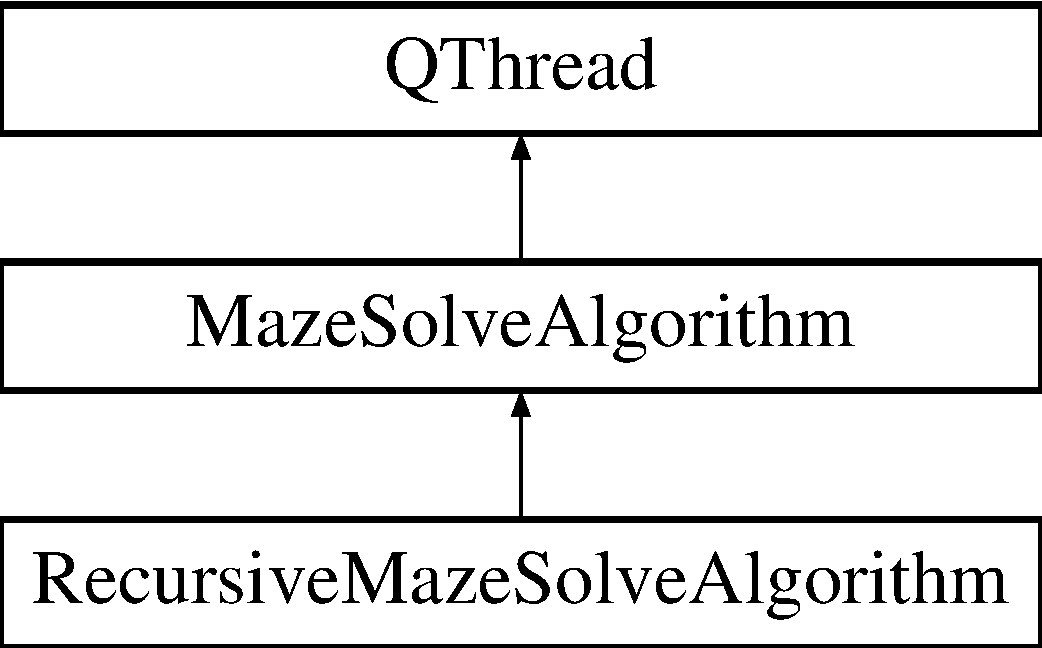
\includegraphics[height=3.000000cm]{class_recursive_maze_solve_algorithm}
\end{center}
\end{figure}
\subsection*{Public Member Functions}
\begin{DoxyCompactItemize}
\item 
\hyperlink{class_recursive_maze_solve_algorithm_a62a60de4fb81a35cae475eabc5a5a66e}{Recursive\-Maze\-Solve\-Algorithm} (\hyperlink{class_maze}{Maze} $\ast$maze)
\begin{DoxyCompactList}\small\item\em \hyperlink{class_recursive_maze_solve_algorithm_a62a60de4fb81a35cae475eabc5a5a66e}{Recursive\-Maze\-Solve\-Algorithm\-::\-Recursive\-Maze\-Solve\-Algorithm} Constructor sets the maze with width, height and startpos. \end{DoxyCompactList}\item 
bool \hyperlink{class_recursive_maze_solve_algorithm_a15c3571e131dffc45ab62a2073aa0da4}{solve} (int \&steps)
\begin{DoxyCompactList}\small\item\em \hyperlink{class_recursive_maze_solve_algorithm_a15c3571e131dffc45ab62a2073aa0da4}{Recursive\-Maze\-Solve\-Algorithm\-::solve} Solves the delivered \hyperlink{class_maze}{Maze}. \end{DoxyCompactList}\end{DoxyCompactItemize}
\subsection*{Additional Inherited Members}


\subsection{Constructor \& Destructor Documentation}
\hypertarget{class_recursive_maze_solve_algorithm_a62a60de4fb81a35cae475eabc5a5a66e}{\index{Recursive\-Maze\-Solve\-Algorithm@{Recursive\-Maze\-Solve\-Algorithm}!Recursive\-Maze\-Solve\-Algorithm@{Recursive\-Maze\-Solve\-Algorithm}}
\index{Recursive\-Maze\-Solve\-Algorithm@{Recursive\-Maze\-Solve\-Algorithm}!RecursiveMazeSolveAlgorithm@{Recursive\-Maze\-Solve\-Algorithm}}
\subsubsection[{Recursive\-Maze\-Solve\-Algorithm}]{\setlength{\rightskip}{0pt plus 5cm}Recursive\-Maze\-Solve\-Algorithm\-::\-Recursive\-Maze\-Solve\-Algorithm (
\begin{DoxyParamCaption}
\item[{{\bf Maze} $\ast$}]{maze}
\end{DoxyParamCaption}
)}}\label{class_recursive_maze_solve_algorithm_a62a60de4fb81a35cae475eabc5a5a66e}


\hyperlink{class_recursive_maze_solve_algorithm_a62a60de4fb81a35cae475eabc5a5a66e}{Recursive\-Maze\-Solve\-Algorithm\-::\-Recursive\-Maze\-Solve\-Algorithm} Constructor sets the maze with width, height and startpos. 


\begin{DoxyParams}{Parameters}
{\em maze} & the maze to solve \\
\hline
{\em width} & width of the maze \\
\hline
{\em height} & height of the maze \\
\hline
\end{DoxyParams}


\subsection{Member Function Documentation}
\hypertarget{class_recursive_maze_solve_algorithm_a15c3571e131dffc45ab62a2073aa0da4}{\index{Recursive\-Maze\-Solve\-Algorithm@{Recursive\-Maze\-Solve\-Algorithm}!solve@{solve}}
\index{solve@{solve}!RecursiveMazeSolveAlgorithm@{Recursive\-Maze\-Solve\-Algorithm}}
\subsubsection[{solve}]{\setlength{\rightskip}{0pt plus 5cm}bool Recursive\-Maze\-Solve\-Algorithm\-::solve (
\begin{DoxyParamCaption}
\item[{int \&}]{steps}
\end{DoxyParamCaption}
)\hspace{0.3cm}{\ttfamily [virtual]}}}\label{class_recursive_maze_solve_algorithm_a15c3571e131dffc45ab62a2073aa0da4}


\hyperlink{class_recursive_maze_solve_algorithm_a15c3571e131dffc45ab62a2073aa0da4}{Recursive\-Maze\-Solve\-Algorithm\-::solve} Solves the delivered \hyperlink{class_maze}{Maze}. 


\begin{DoxyParams}{Parameters}
{\em enable\-\_\-steps} & flag which enables printing after everey step \\
\hline
\end{DoxyParams}
\begin{DoxyReturn}{Returns}
flag if maze could be solved 
\end{DoxyReturn}


Implements \hyperlink{class_maze_solve_algorithm_a3f957367c4afe52d29b0021766a478be}{Maze\-Solve\-Algorithm}.



The documentation for this class was generated from the following files\-:\begin{DoxyCompactItemize}
\item 
/home/travis/build/algdat/blatt-\/2-\/maze/src/ss17/algodat/maze/control/recursive\-\_\-solver/\hyperlink{recursivemazesolvealgorithm_8h}{recursivemazesolvealgorithm.\-h}\item 
/home/travis/build/algdat/blatt-\/2-\/maze/src/ss17/algodat/maze/control/recursive\-\_\-solver/\hyperlink{recursivemazesolvealgorithm_8cpp}{recursivemazesolvealgorithm.\-cpp}\end{DoxyCompactItemize}

\chapter{File Documentation}
\hypertarget{mazealgorithm_8cpp}{\section{/home/travis/build/algdat/blatt-\/2-\/maze/src/ss17/algodat/maze/control/mazealgorithm.cpp File Reference}
\label{mazealgorithm_8cpp}\index{/home/travis/build/algdat/blatt-\/2-\/maze/src/ss17/algodat/maze/control/mazealgorithm.\-cpp@{/home/travis/build/algdat/blatt-\/2-\/maze/src/ss17/algodat/maze/control/mazealgorithm.\-cpp}}
}
{\ttfamily \#include \char`\"{}mazealgorithm.\-h\char`\"{}}\\*

\hypertarget{mazealgorithm_8h}{\section{/home/travis/build/algdat/blatt-\/2-\/maze/src/ss17/algodat/maze/control/mazealgorithm.h File Reference}
\label{mazealgorithm_8h}\index{/home/travis/build/algdat/blatt-\/2-\/maze/src/ss17/algodat/maze/control/mazealgorithm.\-h@{/home/travis/build/algdat/blatt-\/2-\/maze/src/ss17/algodat/maze/control/mazealgorithm.\-h}}
}
{\ttfamily \#include \char`\"{}../model/maze.\-h\char`\"{}}\\*
{\ttfamily \#include $<$Q\-Thread$>$}\\*
\subsection*{Classes}
\begin{DoxyCompactItemize}
\item 
class \hyperlink{class_maze_solve_algorithm}{Maze\-Solve\-Algorithm}
\begin{DoxyCompactList}\small\item\em The Maze\-Algorithm class Baseclass have to be derived by all maze solve algorithm classes contains the datastructures for the maze such as methods to redrow. \end{DoxyCompactList}\end{DoxyCompactItemize}

\hypertarget{mazegenerator_8cpp}{\section{/home/travis/build/algdat/blatt-\/2-\/maze/src/ss17/algodat/maze/control/mazegenerator.cpp File Reference}
\label{mazegenerator_8cpp}\index{/home/travis/build/algdat/blatt-\/2-\/maze/src/ss17/algodat/maze/control/mazegenerator.\-cpp@{/home/travis/build/algdat/blatt-\/2-\/maze/src/ss17/algodat/maze/control/mazegenerator.\-cpp}}
}
{\ttfamily \#include \char`\"{}mazegenerator.\-h\char`\"{}}\\*
{\ttfamily \#include $<$random$>$}\\*

\hypertarget{mazegenerator_8h}{\section{/home/travis/build/algdat/blatt-\/2-\/maze/src/ss17/algodat/maze/control/mazegenerator.h File Reference}
\label{mazegenerator_8h}\index{/home/travis/build/algdat/blatt-\/2-\/maze/src/ss17/algodat/maze/control/mazegenerator.\-h@{/home/travis/build/algdat/blatt-\/2-\/maze/src/ss17/algodat/maze/control/mazegenerator.\-h}}
}
{\ttfamily \#include \char`\"{}maze.\-h\char`\"{}}\\*
\subsection*{Classes}
\begin{DoxyCompactItemize}
\item 
class \hyperlink{class_maze_generator}{Maze\-Generator}
\end{DoxyCompactItemize}

\hypertarget{recursivemazesolvealgorithm_8cpp}{\section{/home/travis/build/algdat/blatt-\/2-\/maze/src/ss17/algodat/maze/control/recursive\-\_\-solver/recursivemazesolvealgorithm.cpp File Reference}
\label{recursivemazesolvealgorithm_8cpp}\index{/home/travis/build/algdat/blatt-\/2-\/maze/src/ss17/algodat/maze/control/recursive\-\_\-solver/recursivemazesolvealgorithm.\-cpp@{/home/travis/build/algdat/blatt-\/2-\/maze/src/ss17/algodat/maze/control/recursive\-\_\-solver/recursivemazesolvealgorithm.\-cpp}}
}
{\ttfamily \#include \char`\"{}recursivemazesolvealgorithm.\-h\char`\"{}}\\*

\hypertarget{recursivemazesolvealgorithm_8h}{\section{/home/travis/build/algdat/blatt-\/2-\/maze/src/ss17/algodat/maze/control/recursive\-\_\-solver/recursivemazesolvealgorithm.h File Reference}
\label{recursivemazesolvealgorithm_8h}\index{/home/travis/build/algdat/blatt-\/2-\/maze/src/ss17/algodat/maze/control/recursive\-\_\-solver/recursivemazesolvealgorithm.\-h@{/home/travis/build/algdat/blatt-\/2-\/maze/src/ss17/algodat/maze/control/recursive\-\_\-solver/recursivemazesolvealgorithm.\-h}}
}
{\ttfamily \#include \char`\"{}mazealgorithm.\-h\char`\"{}}\\*
\subsection*{Classes}
\begin{DoxyCompactItemize}
\item 
class \hyperlink{class_recursive_maze_solve_algorithm}{Recursive\-Maze\-Solve\-Algorithm}
\end{DoxyCompactItemize}

\hypertarget{_breadth_first_search_8cpp}{\section{/home/travis/build/algdat/blatt-\/2-\/maze/src/ss17/algodat/maze/control/shortest\-\_\-path/breadth\-\_\-first\-\_\-search/\-Breadth\-First\-Search.cpp File Reference}
\label{_breadth_first_search_8cpp}\index{/home/travis/build/algdat/blatt-\/2-\/maze/src/ss17/algodat/maze/control/shortest\-\_\-path/breadth\-\_\-first\-\_\-search/\-Breadth\-First\-Search.\-cpp@{/home/travis/build/algdat/blatt-\/2-\/maze/src/ss17/algodat/maze/control/shortest\-\_\-path/breadth\-\_\-first\-\_\-search/\-Breadth\-First\-Search.\-cpp}}
}
{\ttfamily \#include $<$string$>$}\\*
{\ttfamily \#include $<$queue$>$}\\*
{\ttfamily \#include \char`\"{}Breadth\-First\-Search.\-h\char`\"{}}\\*
{\ttfamily \#include \char`\"{}Breadth\-First\-Search\-Lib.\-h\char`\"{}}\\*

\hypertarget{_breadth_first_search_8h}{\section{/home/travis/build/algdat/blatt-\/2-\/maze/src/ss17/algodat/maze/control/shortest\-\_\-path/breadth\-\_\-first\-\_\-search/\-Breadth\-First\-Search.h File Reference}
\label{_breadth_first_search_8h}\index{/home/travis/build/algdat/blatt-\/2-\/maze/src/ss17/algodat/maze/control/shortest\-\_\-path/breadth\-\_\-first\-\_\-search/\-Breadth\-First\-Search.\-h@{/home/travis/build/algdat/blatt-\/2-\/maze/src/ss17/algodat/maze/control/shortest\-\_\-path/breadth\-\_\-first\-\_\-search/\-Breadth\-First\-Search.\-h}}
}
{\ttfamily \#include $<$queue$>$}\\*
{\ttfamily \#include \char`\"{}Position.\-h\char`\"{}}\\*
{\ttfamily \#include \char`\"{}../../../model/maze.\-h\char`\"{}}\\*
\subsection*{Classes}
\begin{DoxyCompactItemize}
\item 
class \hyperlink{class_breadth_first_search}{Breadth\-First\-Search}
\begin{DoxyCompactList}\small\item\em Algorithm to find shortest way through maze by using breadth fist search. \end{DoxyCompactList}\end{DoxyCompactItemize}

\hypertarget{_breadth_first_search_gui_interaction_8cpp}{\section{/home/travis/build/algdat/blatt-\/2-\/maze/src/ss17/algodat/maze/control/shortest\-\_\-path/breadth\-\_\-first\-\_\-search/\-Breadth\-First\-Search\-Gui\-Interaction.cpp File Reference}
\label{_breadth_first_search_gui_interaction_8cpp}\index{/home/travis/build/algdat/blatt-\/2-\/maze/src/ss17/algodat/maze/control/shortest\-\_\-path/breadth\-\_\-first\-\_\-search/\-Breadth\-First\-Search\-Gui\-Interaction.\-cpp@{/home/travis/build/algdat/blatt-\/2-\/maze/src/ss17/algodat/maze/control/shortest\-\_\-path/breadth\-\_\-first\-\_\-search/\-Breadth\-First\-Search\-Gui\-Interaction.\-cpp}}
}
{\ttfamily \#include \char`\"{}Breadth\-First\-Search\-Gui\-Interaction.\-h\char`\"{}}\\*

\hypertarget{_breadth_first_search_gui_interaction_8h}{\section{/home/travis/build/algdat/blatt-\/2-\/maze/src/ss17/algodat/maze/control/shortest\-\_\-path/breadth\-\_\-first\-\_\-search/\-Breadth\-First\-Search\-Gui\-Interaction.h File Reference}
\label{_breadth_first_search_gui_interaction_8h}\index{/home/travis/build/algdat/blatt-\/2-\/maze/src/ss17/algodat/maze/control/shortest\-\_\-path/breadth\-\_\-first\-\_\-search/\-Breadth\-First\-Search\-Gui\-Interaction.\-h@{/home/travis/build/algdat/blatt-\/2-\/maze/src/ss17/algodat/maze/control/shortest\-\_\-path/breadth\-\_\-first\-\_\-search/\-Breadth\-First\-Search\-Gui\-Interaction.\-h}}
}
{\ttfamily \#include \char`\"{}../../mazealgorithm.\-h\char`\"{}}\\*
{\ttfamily \#include \char`\"{}Breadth\-First\-Search.\-h\char`\"{}}\\*
{\ttfamily \#include $<$queue$>$}\\*
{\ttfamily \#include $<$string.\-h$>$}\\*
{\ttfamily \#include \char`\"{}Position.\-h\char`\"{}}\\*
{\ttfamily \#include \char`\"{}../../../model/maze.\-h\char`\"{}}\\*
{\ttfamily \#include $<$cstring$>$}\\*
\subsection*{Classes}
\begin{DoxyCompactItemize}
\item 
class \hyperlink{class_breadth_first_search_gui_interaction}{Breadth\-First\-Search\-Gui\-Interaction}
\begin{DoxyCompactList}\small\item\em Wraps logic of Breath\-First\-Search into class extending \hyperlink{class_maze_solve_algorithm}{Maze\-Solve\-Algorithm}. \end{DoxyCompactList}\end{DoxyCompactItemize}

\hypertarget{_position_8cpp}{\section{/home/travis/build/algdat/blatt-\/2-\/maze/src/ss17/algodat/maze/control/shortest\-\_\-path/breadth\-\_\-first\-\_\-search/\-Position.cpp File Reference}
\label{_position_8cpp}\index{/home/travis/build/algdat/blatt-\/2-\/maze/src/ss17/algodat/maze/control/shortest\-\_\-path/breadth\-\_\-first\-\_\-search/\-Position.\-cpp@{/home/travis/build/algdat/blatt-\/2-\/maze/src/ss17/algodat/maze/control/shortest\-\_\-path/breadth\-\_\-first\-\_\-search/\-Position.\-cpp}}
}
{\ttfamily \#include \char`\"{}Position.\-h\char`\"{}}\\*

\hypertarget{_position_8h}{\section{/home/travis/build/algdat/blatt-\/2-\/maze/src/ss17/algodat/maze/control/shortest\-\_\-path/breadth\-\_\-first\-\_\-search/\-Position.h File Reference}
\label{_position_8h}\index{/home/travis/build/algdat/blatt-\/2-\/maze/src/ss17/algodat/maze/control/shortest\-\_\-path/breadth\-\_\-first\-\_\-search/\-Position.\-h@{/home/travis/build/algdat/blatt-\/2-\/maze/src/ss17/algodat/maze/control/shortest\-\_\-path/breadth\-\_\-first\-\_\-search/\-Position.\-h}}
}
{\ttfamily \#include $<$string$>$}\\*
\subsection*{Classes}
\begin{DoxyCompactItemize}
\item 
class \hyperlink{class_position}{Position}
\end{DoxyCompactItemize}

\hypertarget{main_8cpp}{\section{/home/travis/build/algdat/blatt-\/2-\/maze/src/ss17/algodat/maze/main.cpp File Reference}
\label{main_8cpp}\index{/home/travis/build/algdat/blatt-\/2-\/maze/src/ss17/algodat/maze/main.\-cpp@{/home/travis/build/algdat/blatt-\/2-\/maze/src/ss17/algodat/maze/main.\-cpp}}
}
{\ttfamily \#include \char`\"{}mazegui.\-h\char`\"{}}\\*
{\ttfamily \#include $<$Q\-Application$>$}\\*
\subsection*{Functions}
\begin{DoxyCompactItemize}
\item 
int \hyperlink{main_8cpp_a0ddf1224851353fc92bfbff6f499fa97}{main} (int argc, char $\ast$argv\mbox{[}$\,$\mbox{]})
\end{DoxyCompactItemize}


\subsection{Function Documentation}
\hypertarget{main_8cpp_a0ddf1224851353fc92bfbff6f499fa97}{\index{main.\-cpp@{main.\-cpp}!main@{main}}
\index{main@{main}!main.cpp@{main.\-cpp}}
\subsubsection[{main}]{\setlength{\rightskip}{0pt plus 5cm}int main (
\begin{DoxyParamCaption}
\item[{int}]{argc, }
\item[{char $\ast$}]{argv\mbox{[}$\,$\mbox{]}}
\end{DoxyParamCaption}
)}}\label{main_8cpp_a0ddf1224851353fc92bfbff6f499fa97}

\hypertarget{maze_8cpp}{\section{/home/travis/build/algdat/blatt-\/2-\/maze/src/ss17/algodat/maze/model/maze.cpp File Reference}
\label{maze_8cpp}\index{/home/travis/build/algdat/blatt-\/2-\/maze/src/ss17/algodat/maze/model/maze.\-cpp@{/home/travis/build/algdat/blatt-\/2-\/maze/src/ss17/algodat/maze/model/maze.\-cpp}}
}
{\ttfamily \#include \char`\"{}maze.\-h\char`\"{}}\\*

\hypertarget{maze_8h}{\section{/home/travis/build/algdat/blatt-\/2-\/maze/src/ss17/algodat/maze/model/maze.h File Reference}
\label{maze_8h}\index{/home/travis/build/algdat/blatt-\/2-\/maze/src/ss17/algodat/maze/model/maze.\-h@{/home/travis/build/algdat/blatt-\/2-\/maze/src/ss17/algodat/maze/model/maze.\-h}}
}
{\ttfamily \#include $<$mutex$>$}\\*
\subsection*{Classes}
\begin{DoxyCompactItemize}
\item 
class \hyperlink{class_maze}{Maze}
\begin{DoxyCompactList}\small\item\em The \hyperlink{class_maze}{Maze} class contains the model of the maze with functions to set an get fields of the maze. \end{DoxyCompactList}\end{DoxyCompactItemize}

\hypertarget{mazegui_8cpp}{\section{/home/travis/build/algdat/blatt-\/2-\/maze/src/ss17/algodat/maze/view/mazegui.cpp File Reference}
\label{mazegui_8cpp}\index{/home/travis/build/algdat/blatt-\/2-\/maze/src/ss17/algodat/maze/view/mazegui.\-cpp@{/home/travis/build/algdat/blatt-\/2-\/maze/src/ss17/algodat/maze/view/mazegui.\-cpp}}
}
{\ttfamily \#include \char`\"{}mazegui.\-h\char`\"{}}\\*
{\ttfamily \#include \char`\"{}ui\-\_\-mazegui.\-h\char`\"{}}\\*
{\ttfamily \#include \char`\"{}mazegenerator.\-h\char`\"{}}\\*
{\ttfamily \#include $<$control/shortest\-\_\-path/breadth\-\_\-first\-\_\-search/\-Breadth\-First\-Search.\-h$>$}\\*

\hypertarget{mazegui_8h}{\section{/home/travis/build/algdat/blatt-\/2-\/maze/src/ss17/algodat/maze/view/mazegui.h File Reference}
\label{mazegui_8h}\index{/home/travis/build/algdat/blatt-\/2-\/maze/src/ss17/algodat/maze/view/mazegui.\-h@{/home/travis/build/algdat/blatt-\/2-\/maze/src/ss17/algodat/maze/view/mazegui.\-h}}
}
{\ttfamily \#include $<$Q\-Main\-Window$>$}\\*
{\ttfamily \#include $<$Q\-Dialog$>$}\\*
{\ttfamily \#include $<$Qt\-Core$>$}\\*
{\ttfamily \#include $<$Qt\-Gui$>$}\\*
{\ttfamily \#include $<$Q\-Graphics\-Scene$>$}\\*
{\ttfamily \#include $<$Q\-Graphics\-Rect\-Item$>$}\\*
{\ttfamily \#include $<$vector$>$}\\*
{\ttfamily \#include $<$qmainwindow.\-h$>$}\\*
{\ttfamily \#include \char`\"{}recursivemazesolvealgorithm.\-h\char`\"{}}\\*
{\ttfamily \#include \char`\"{}maze.\-h\char`\"{}}\\*
\subsection*{Classes}
\begin{DoxyCompactItemize}
\item 
class \hyperlink{class_maze_gui}{Maze\-Gui}
\end{DoxyCompactItemize}
\subsection*{Namespaces}
\begin{DoxyCompactItemize}
\item 
\hyperlink{namespace_ui}{Ui}
\end{DoxyCompactItemize}

%--- End generated contents ---

% Index
\newpage
\phantomsection
\addcontentsline{toc}{chapter}{Index}
\printindex

\end{document}
